We extensively covered the mechanism of (multiverse-wide)
superrationality. However, in all thought experiments considered so far,
we knew what impact our actions would have on the fulfillment of the
other agents' preferences. For example, we know that the other
participants in the donation game or Platonia five would prefer to have
more money on their bank account. We also know that other civilizations
would prefer not to be destroyed in
\ref{hierarchies-and-acyclic-graphs} and would benefit from learning about our technologies. Such
knowledge has to be present or at least attainable in the future (cf.
section
\ref{cooperation-in-the-face-of-uncertainty-about-values}),
otherwise no side can benefit the others. This section gives an overview
of how we can find out what other agents in the multiverse care about,
as well as what aspects of their preferences we should focus on in the
first place.

\hypertarget{orthogonality-of-instrumental-rationality-and-values}{\subsection{Orthogonality
of instrumental rationality and
values}\label{orthogonality-of-instrumental-rationality-and-values}}

One objection to superrational cooperation might be based on a possible
convergence of terminal values, in which all agents with the correct
decision theory will converge toward the same values.
\href{https://en.wikipedia.org/wiki/Moral_realism}{\emph{Moral realism}}
claims that there are facts in morality as real and true as those in
science. In addition, some moral realists believe that any rational
agent investigating morality will ultimately arrive at these moral
truths. Assuming that a large part of being rational involves using the
right decision theory, maybe all agents with the right decision theory
will independently come to adopt the ``correct'' moral system? If this
is the case, no cooperation among these agents would be necessary
(although some value systems may still require multiverse-wide
\ref{notes-on-superrational-coordination},
see section
\ref{notes-on-superrational-coordination}).

As a first counterargument, consider that knowledge of the
\emph{correct} decision is not necessary for superrational cooperation,
seeing as a
\href{https://casparoesterheld.com/a-comprehensive-list-of-decision-theories/}{\emph{number
of different decision theories}} (e.g.,
\href{https://en.wikipedia.org/wiki/Evidential_decision_theory}{\emph{evidential}},
\href{https://intelligence.org/files/TDT.pdf}{\emph{timeless}} and
\href{https://wiki.lesswrong.com/wiki/Updateless_decision_theory}{\emph{updateless}}
decision theory) imply superrationality. Secondly, we do not seem to
observe empirical evidence of such convergence. For example, Eliezer
Yudkowsky and Brian Tomasik agree that non-causal considerations are
important for decision theory, but
\href{https://wiki.lesswrong.com/wiki/Fun_theory}{\emph{Yudkowsky's
values}} nevertheless differ significantly from
\href{http://reducing-suffering.org/\#Ethics}{\emph{Tomasik's}}.

There are also principled reasons to be skeptical of value convergence
among agents with the same decision theory. Decision theories are about
\emph{instrumental rationality}, i.e. about making decisions aimed at
achieving goals, not at revising them\footnote{Apparently, some authors
  \href{https://en.wikipedia.org/wiki/Instrumental_and_value_rationality}{\emph{differentiate}}
  between instrumental and ``value rationality''. I would probably
  disagree with the assumptions underlying the use of the term ``value
  rationality'' (see footnote \ref{non-cognitivism}).
  Nevertheless, I agree with the differentiation itself.}. That is at
least the case for decision theories as they are discussed today.
Consider the following variant of the donation game:

\begin{quote}
\textbf{Donation game for sadists.} Omega has selected 20 \emph{pure
sadists}, who draw pleasure only from torturing others and nothing else.
They all use similar decision making mechanisms when playing a donation
game (against correlated agents). Instead of being paid in dollar sums,
they are given individual hours to torture a slave as a reward.
\end{quote}

Assuming sufficient correlation between participants, the instrumentally
rational decision for each sadist is to cooperate such that the total
number of hours of torture increases relative to universal defection.
The moral choice, on the other hand, would be to defect in order to
reduce the number of hours in which anyone gets tortured. However,
decision theories (as currently discussed in the literature) do not take
moral considerations into account at all. They merely aim to fulfill the
goals, whatever they may be, of the agent using that decision theory.
Hence, when applied by a pure sadist, a given decision theory is meant
to help her spend more time torturing others.\footnote{In most human
  sadists, sadism is probably not the only goal or cause of happiness.
  Many sadists probably recognize their urges as morally wrong, yet are
  unable to control them to varying degrees. To these sadists, a
  decision theory may provide a nudge towards seeking professional help
  (at least if they cannot satisfy their sadistic preferences in morally
  nonproblematic ways).}

There could conceivably be some different kind of ``decision theory''
that does recommend taking morality into account (and not only
cooperation, see section \ref{real-altruism}) even if the agent using it is amoral or immoral. One
could, for instance, simply combine the correct decision theory with the
``correct'' moral view. Some people may consider such a decision theory
objectively correct. However, for an agent with immoral goals (like pure
sadism), it
\href{http://reducing-suffering.org/thoughts-on-postmodernism-and-its-intellectual-kin/\#Why_care_about_ethics}{\emph{would
be}} instrumentally \emph{irrational} to adopt such a decision theory.
In any case, the existence of such a ``moral decision theory'' does not
contradict the existence of a decision theory in the classical,
instrumentally rational sense, so an amoral or immoral agent would still
be better off adopting a classical decision theory.

Thus, it would seem that an agent's values and their use of acausal
decision theories are orthogonal. This, in turn, suggests that agents
with a variety of value systems will adopt a decision theory similar to
our own, such that their decisions will correlate with ours.

Similar views regarding the relationship between
\href{http://lesswrong.com/lw/31/what_do_we_mean_by_rationality/}{\emph{instrumental
(and epistemic) rationality}} and ethical values have been defended
under the term \emph{orthogonality thesis}
\parencite{Bostrom2014-pc,Bostrom2012-hj,Armstrong2013-xo}.

Our claim that decision theory and values are orthogonal in principle
does not imply that they never correlate in practice throughout the
multiverse. Indeed, in section
\ref{the-values-of-our-superrational-collaborators-in-the-multiverse} and its
companion papers, I will discuss various ways in which values and
decision algorithms could be expected to correlate. However, it seems
very unlikely to me that these correlations are so strong that they
significantly dampen the relevance of superrationality.

\hypertarget{necessary-preconditions}{\subsection{Necessary
preconditions}\label{necessary-preconditions}}

Before we start thinking about the values of agents in other parts of
the multiverse, we need to consider what kind of agents can join
multiverse-wide superrational cooperation (MSR) at all. In particular,
what sorts of values do they need to have, independent of whether or how
many such agents or value systems actually exist in the multiverse? We
already know that only helping superrational or correlated agents
benefits us (see section
\ref{only-helping-superrational-cooperators-helps-you-superrationally}).
However, the values of the superrationalists must also be open to the
opportunity of gains from compromise. If an agent's values imply that
she is better off without any trades, there is no point in helping her.
In order to more closely examine this precondition, we can break it into
five distinct criteria, all of which are necessary for a superrational
collaborator to reap the gains from compromise.

\begin{enumerate}
\def\labelenumi{\arabic{enumi}.}
\item
  Each collaborator must care to at least some extent about states of
  the world, as opposed to caring only about their own mental states or
  actions.
\item
  They must also care about consequences in areas of the multiverse
  where there may be other cooperators.
\item
  Other superrationalists must be able to infer and understand their
  values in sufficient detail. (To draw action-guiding conclusions from
  MSR, they themselves need to be able to infer the values of some other
  superrationalists or to influence future agents with this ability.)
\item
  Given this knowledge of their values, collaborators must have some
  power to behave nicely toward this value systems. (Again, if MSR is to
  be action-guiding to an agent, they in turn need to be able to benefit
  other values.)
\item
  Doing so produces gains from compromise. If everyone abides by an
  analogous cooperative strategy, everyone is better off than they would
  be without cooperation.
\end{enumerate}

If all these criteria are satisfied, superrational cooperation works. We
will discuss the first five criteria in the following sections. The
sixth is discussed in section
\ref{only-helping-superrational-cooperators-helps-you-superrationally}.

For some applications it may be fruitful to subdivide these criteria
further. Furthermore, additional criteria, such as
\parencite{Bostrom2014-gy} ``porosity'', may determine the
size of the gains from compromise. We could furthermore devise criteria
to assess the extent to which superrational cooperation affects one's
strategy. For instance, if all correlated agents have the same values
anyway, superrational cooperation does not affect our policy except for
cases of coordination (see section
\ref{notes-on-superrational-coordination}).

\hypertarget{consequentialism}{\subsubsection{Consequentialism}\label{consequentialism}}

Most people's ethical views are partly
\href{https://en.wikipedia.org/wiki/Deontological_ethics}{\emph{deontological}}
(and sometimes
\href{https://en.wikipedia.org/wiki/Virtue_ethics}{\emph{virtue
ethical}}). That is, they are not solely concerned about the state of
the world and the consequences of actions, but als about ``the actions
themselves'' (and, in case of virtue ethics, one's character). They
usually try to follow some set of rules prescribing what actions are
appropriate in which situations. For example, many people follow strict
rules against killing (though these usually do not apply under all
circumstances and the meaning of ``killing'' is rarely fully specified),
even when breaking these rules would lead to fewer deaths. This type of
ethical system forms a central part of many religious doctrines, with
notable examples such as the Christian ten commandments, the
\href{https://en.wikipedia.org/wiki/Ten_Commandments}{C}o\href{https://en.wikipedia.org/wiki/Ten_Commandments}{n}f\href{https://en.wikipedia.org/wiki/Ten_Commandments}{u}c\href{https://en.wikipedia.org/wiki/Ten_Commandments}{i}a\href{https://en.wikipedia.org/wiki/Ten_Commandments}{n}
\href{https://en.wikipedia.org/wiki/Filial_piety}{\emph{filial
piety}}\href{https://en.wikipedia.org/wiki/Ten_Commandments}{,} and
Islamic sharia. In addition, most national laws contain countless rules
of this sort, many of which apply to more mundane domains like traffic
or taxes. Isaac Asimov's
\href{https://en.wikipedia.org/wiki/Three_Laws_of_Robotics}{\emph{three
laws of robotics}} are yet another example of a deontological set of
rules.

The arguments for multiverse-wide superrational cooperation that I have
given appeal to the
\href{https://en.wikipedia.org/wiki/Consequentialism}{\emph{consequentialist}}
aspects of one's values -- not because it requires us to push people off
bridges (as in the
\href{https://en.wikipedia.org/wiki/Trolley_problem\#The_fat_man}{\emph{Fat
man version of the Trolley problem}}), but because its supporting
argument is fundamentally based on the consequences of different
actions. If we on Earth benefit other value systems, then this implies
that others elsewhere in the multiverse also benefit our value system,
which may produce better overall states of the multiverse overall via
\href{https://foundational-research.org/gains-from-trade-through-compromise/}{\emph{gains
from trade}}. Hence, the value of superrational cooperation lies in its
positive consequences on the world (or other worlds). The ethical duties
of deontological ethical systems, on the other hand, usually concern the
more immediate consequences of our actions. Thus, in a scenario like the
Fat man version of the Trolley problem, most deontological would imply
that the direct act of killing the fat man violates our duties towards
him more than a failure to act violates our duty towards the five people
on the track.

In Bourget and Chalmers' survey of philosophers \parencite{Bourget2014-fm}, 23.6\%
of respondents characterized their values as consequentialist while
44.1\% identified as deontologists or virtue ethicists -- with the
remaining 32.3\% choosing ``other''. However, most people probably
espouse values that involve at least some consequentialist aspects (cf.
\cite{Muehlhauser2012-ib}). I doubt that many modern
consequentialists would be emotionally capable of murder or torture even
under circumstances where they could be confident that doing so would
yield the best consequences\footnote{In my personal experience,
  self-identified consequentialists actually tend to be more virtue
  ethical in their behavior than the average person.}. At the same time,
I doubt that many defendants of rule-based ethics see no appeal in
potentially reducing the amount of torture in the multiverse, even if
only in an indirect way. In fact, many deontological rules are motivated
or even defined by the consequences they produce. For example, murder is
defined as any act that intentionally and directly results in the death
of another person (although indirect ways of causing the same
consequence (e.g.,
\href{https://en.wikipedia.org/wiki/Omission_bias}{\emph{omissions}})
are not seen as murder). Rules against theft are often defended on the
grounds that a society with such rules is preferable to one without,
even if the rules might occasionally prevent a genuinely altruistic bank
robbery. Some even
\href{http://briantomasik.com/interpreting-the-categorical-imperative/\#Categorical_imperative_as_decision_theory}{\emph{interpret}}
Kant's
\href{https://en.wikipedia.org/wiki/Categorical_imperative}{\emph{categorical
imperative}} (especially its first ``formulation'') as a heuristic based
on consequentially motivated decision-theoretical reasoning
\parencite{Parfit2011-xj,Hare1993-gi}. As
writes, ``deontological theories
are {[}not defined{]} as views that characterize the rightness of
institutions and acts independently from their consequences. All ethical
doctrines worth our attention take consequences into account in judging
rightness. One which did not would simply be irrational, crazy.''
\parencite{Rawls1971-sq} Although most people refrain from the consequentialist choice in extreme
situations, they do, in fact, often endorse it. For example, in
Bourget and Chalmers' survey \parencite{Bourget2014-fm}, 68.2\% of the respondents
chose to pull the switch in the original
\href{https://en.wikipedia.org/wiki/Trolley_problem}{\emph{trolley
problem}}, and only 7.6\% did not (with the remaining 24.2\% choosing
``other''). Pulling the switch
\href{https://en.wikipedia.org/wiki/Trolley_problem\#Psychology}{\emph{is
similarly popular}} among the general population. This suggests that
people sometimes agree with consequentialist reasoning even if other,
exclusively deontological or virtue ethical considerations can overrule
it.

Beyond consequences for things like the number of deaths, individual
welfare, and fairness, people sometimes also care about the abidance by
deontological rules in a consequentialist way. For example, most people
not only avoid killing others themselves, but also care about preventing
murders in general; many who personally avoid lying also strongly
dislike it when others lie; and so forth. These kinds of
consequentialism, which are rarely considered in the literature on moral
philosophy, qualify for superrational consideration just as much as,
say,
\href{https://en.wikipedia.org/wiki/Utilitarianism}{\emph{utilitarianism}}.
We will revisit this topic of caring about the deontologically ethical
behavior of others in section
\ref{human-far-values}, in
which we review studies indicating that many people have values of this
sort.

\hypertarget{caring-about-the-multiverse}{\subsubsection{Caring about
the multiverse}\label{caring-about-the-multiverse}}

Presumably, some agents with significant consequentialist aspects to
their values will almost exclusively care about their own part of the
multiverse, if only based on
\href{https://en.wikipedia.org/wiki/Ethical_egoism}{\emph{egoism}} or
\href{https://wiki.lesswrong.com/wiki/Absurdity_heuristic}{\emph{absurdity
heuristics}}\footnote{One may argue that absurdity heuristics are a part
  of someone's
  \href{https://en.wikipedia.org/wiki/Epistemology}{\emph{epistemology}}.
  That is, the ``absurdity'' of the Everett interpretation is used as a
  reason to give it low probability as a theory of physics. However, it
  \href{http://reducing-suffering.org/why-does-physics-exist/\#My_new_understanding}{\emph{is
  not clear}} whether there is a clear-cut, operational difference
  between belief and preference if the belief does not make a testable
  prediction.}. It is thus very difficult or impossible to benefit them
in other parts of the multiverse, in turn preventing cooperation.

Although there is very little discussion about the moral relevance of
other parts of the multiverse, the moral relevance of distance is
frequently discussed in moral philosophy (see, e.g.,
\cite{Brock2013-cv}. Note that while distance is
usually understood to be spatial, other kinds of distance (e.g.,
\href{https://sentience-politics.org/philosophy/the-importance-of-the-future/}{\emph{temporal}}
\parencite{Beckstead2013-lv} or social) play similar roles
in ethical judgment.

While the debate in moral philosophy appears ambiguous, people's actions
speak more clearly. Most people from high-income countries would save a
child from drowning in a nearby pond, but donate
\href{http://nccs.urban.org/nccs/statistics/charitable-giving-in-america-some-facts-and-figures.cfm}{\emph{only
relatively small}} amounts to charity
\parencite{Singer1972-uk}. Insofar as they do give to
charity, they usually prefer local causes even though helping in
low-income countries
\href{http://www.givewell.org/giving101/Your-dollar-goes-further-overseas}{\emph{is}}
more cost-effective. From this, we can safely infer that most people are
altruistic to some extent, but seem to care more about near events
rather than distant ones.

One may suspect that an agent's ignorance about other parts of the
multiverse would yield similar conclusions as a lack of interest. After
all, if someone does not know about our part of the multiverse, they
cannot help us. However, we must not forget that superrational
cooperation need not be based on mutuality (see section
\ref{no-reciprocity-needed-whom-to-treat-beneficially}). Even if someone
cannot help us, we can still help them to make it more likely that we
ourselves receive help from agents whom \emph{we} cannot help.

\subsubsection{Knowable values}\label{knowable-values}

In order to maximize for some given utility function, we or future
superrationalists (see section
\ref{cooperation-in-the-face-of-uncertainty-about-values}) need a
sufficiently detailed model of the utility function itself. In section
\ref{the-values-of-our-superrational-collaborators-in-the-multiverse}, we will discuss how the
evolutionary psychology of morality and related disciplines can be used to assess the values of
superrational cooperators in the multiverse. There are at least some ways of making very educated
guesses, although we cannot expect to arrive at a detailed and precise description of the values of
all evolved civilizations and their descendants. However, perfect knowledge is not necessary for our
purposes. Indeed, most people cannot even describe their own values in detail (see footnote
\ref{we-do-not-know-our-utility-function}). Yet despite this, humans are perfectly capable of
helping one another achieve their goals. Thus, the question is neither whether we can gain relevant
knowledge about the values of other agents in the multiverse at all, nor whether we can have a full
map of extraterrestrial morality, but whether the information we can gather about other
civilizations can be \emph{sufficiently} accurate to yield a usable model.

\hypertarget{fragility-of-value}{\paragraph{Fragility of
value}\label{fragility-of-value}}

Eliezer Yudkowsky \parencite{Yudkowsky2015-tz} argues that human
values are not just complex (cf. section
\ref{organizing-human-values});
they are also fragile, in the sense that even minor errors in a
non-human agent's picture of them can completely derail that agent's
efforts to optimize for them. According to Yudkowsky, ``Any Future not
shaped by a goal system with detailed reliable inheritance from human
morals and metamorals, will contain almost nothing of worth.'' Perhaps
more generally, we could say that any resource expenditure will generate
next to no value for an intelligent evolved being X unless that resource
expenditure is shaped by a detailed inheritance of X's morals and
metamorals. Yudkowsky gives boredom as an example of a small but
indispensable part of human values:

\begin{quote}
``Consider the
\href{http://lesswrong.com/lw/xr/in_praise_of_boredom/}{\emph{incredibly
important human value of `boredom'}} -- our desire not to do `the same
thing' over and over and over again. You can imagine a mind that
contained almost the whole specification of human value, almost all the
morals and metamorals, but left out just this one thing and so it spent
until the end of time, and until the farthest reaches of its light cone,
replaying a single highly optimized experience, over and over and over
again.''
\end{quote}

Presumably, many other seemingly insignificant aspects of human values
are of similar importance as boredom. One would need to get all of these
aspects just right in order to benefit human values. This suggests that
it will be difficult to benefit many evolved value systems, due to the
large amount of detailed knowledge it would require and the difficulty
of gathering that knowledge.

There are various points to discuss in this context. For one, the
fragility thesis is rather vague; it does not say \emph{how} fragile our
values are, or \emph{how} accurate and reliable the inheritance must be.
This is not to say that the fragility thesis makes no testable claim at
all. Yudkowsky formulated it with the
\href{http://lesswrong.com/lw/llr/superintelligence_20_the_valueloading_problem/}{\emph{value
loading problem of artificial intelligence}} in mind. Since AIs can be
programmed to pursue any goal (cf. section
\ref{orthogonality-of-instrumental-rationality-and-values}), the space of possible
values with which an AI could end up is vast, and the target goal
systems occupy only a small fraction of this space. The fragility
hypothesis can be interpreted as one elaboration on just how small this
part of value space is, and how catastrophic it would be (from the
perspective of that value system) to miss it by even a small margin. In
other words: even if we take care to represent all of the most central
aspects of our values (e.g., ``increase the welfare of sentient beings''
or ``reduce inequality'') in the goal system of an AI, the outcome may
still be as bad as an entirely random one if we omit seemingly
peripheral values such as boredom.

Although I agree with the fragility thesis as a descriptive (rather than
normative) statement about human values, I do not think human values are
quite as fragile as Yudkowsky writes. Specifically, I think the outcomes
brought about by AIs with two different goal systems can differ
enormously in their overall worth even if both miss important aspects of
human values. For example, Yudkowsky's hypothetical world full of
repetitive happiness may be boring, but it is still much better than a
world full of suffering, unethical behavior, etc. and nothing of worth
to compensate. But perhaps this judgment is influenced by my own values
(which are mostly about ensuring the welfare of sentient beings with a
strong priority for preventing their
\href{https://foundational-research.org/the-case-for-suffering-focused-ethics/}{\emph{suffering}}),
to the point where it would not generalize to how other humans, or other
evolved agents in general, would view the situation. Transferred to our
variant of the fragility thesis, this nevertheless suggests that even if
we miss significant parts of the values of other superrational
cooperators, taking their values into account may still make a big
difference to them.

More importantly, AI value loading differs significantly from our
attempt to benefit agents in other parts of the multiverse. The main
problem of AI value loading is getting the AI to care intrinsically
about human values. MSR, on the other hand, already gives us the sincere
(instrumental) goal of helping other agents, which the AI lacks. If
anything, we lack \emph{knowledge} of the others' values, whereas AIs
\href{http://lesswrong.com/lw/igf/the_genie_knows_but_doesnt_care/}{\emph{may}}
still not care about them even with perfect knowledge of their values.

Another crucial difference between these two contexts is that in AI
value loading, we usually want the AI to hold the values of one
particular species or group of people. In contrast, when cooperating
superrationally, it is sufficient to know that we benefit many other
superrational agents. We do not need to know whether we benefit some
\emph{particular} species. The extent to which this makes our job easier
depends on how evolved value systems are distributed over value space.
Perhaps they form a few (or many) very small clusters, as depicted in
Figure \ref{map-of-value-space-with-clusters}.
(Needless to say, Figure
\ref{map-of-value-space-with-clusters} is not meant to
be an accurate map of value space. The placements on the map have no
factual basis.)

\begin{figure}[h!]
    \centering
    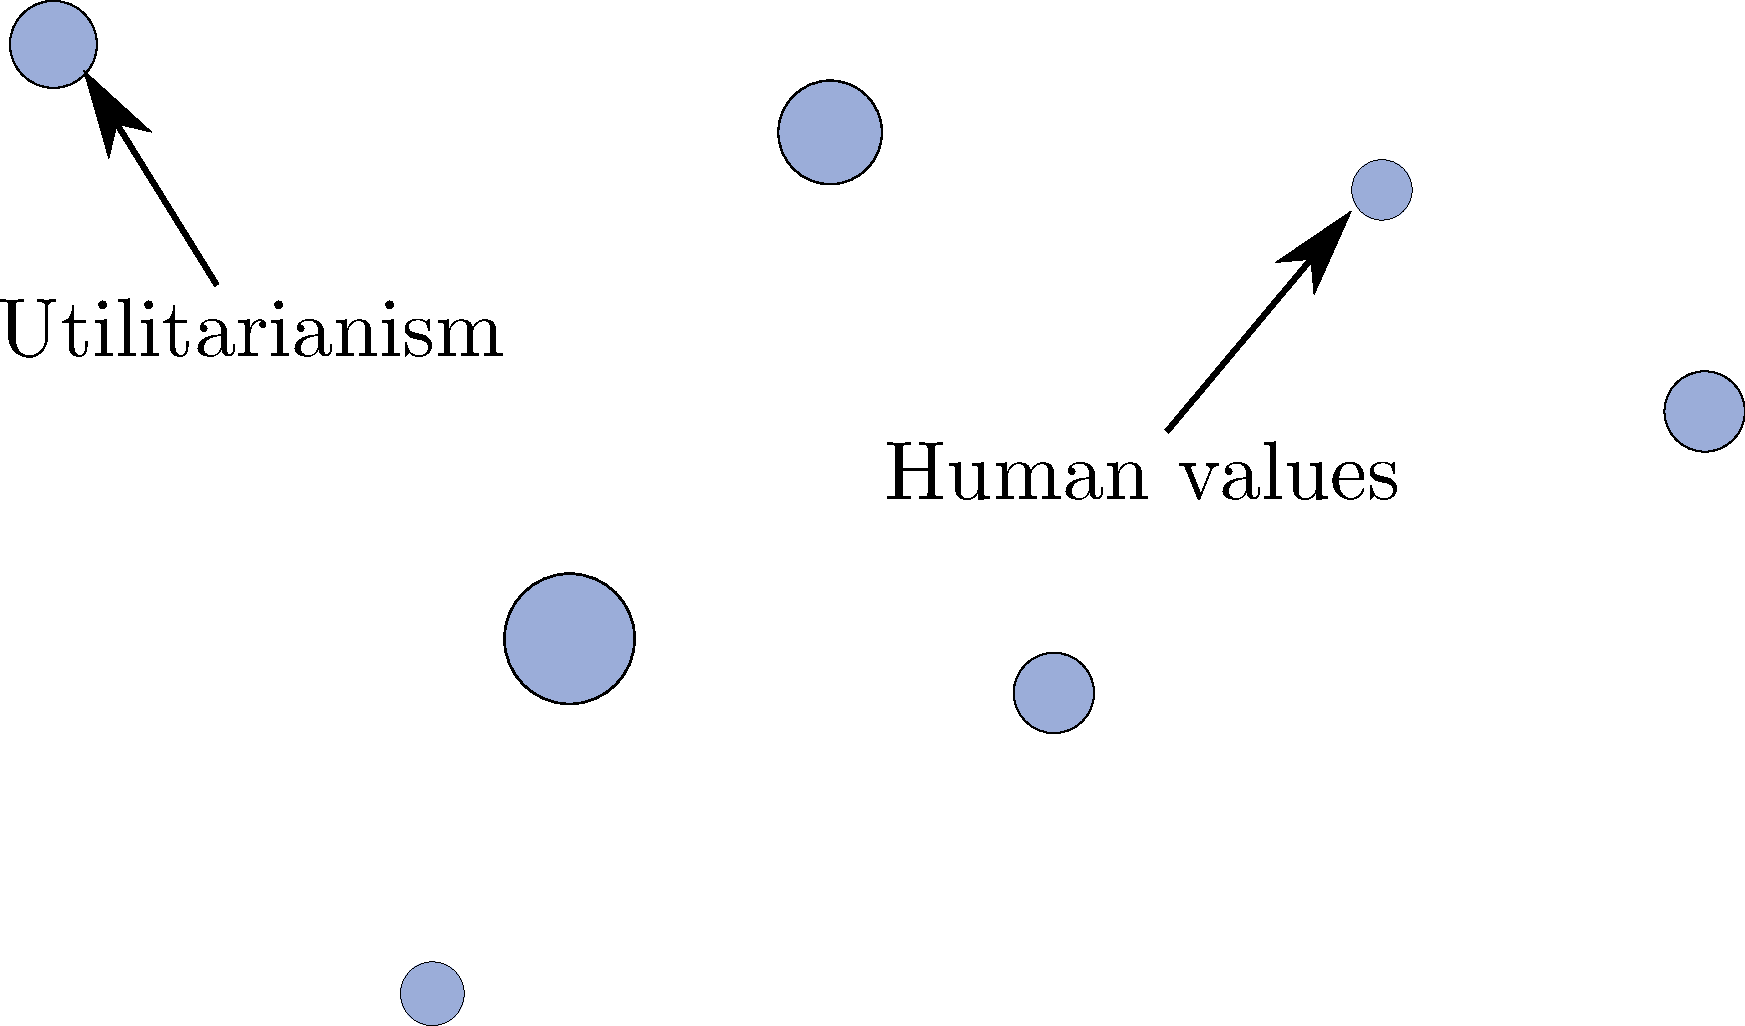
\includegraphics[width=3.21875in,height=2.54167in]{figs/map-of-value-space-with-clusters}
    \caption{A map of a part of value
space under the assumption of there being distinct clusters with a lot
of empty space in between.}
    \label{map-of-value-space-with-clusters}
\end{figure}

Every blue point on the map is some value system held by a significant
number of agents. The white areas of the map contain value systems that
do not have a significant following, such as
\href{https://wiki.lesswrong.com/wiki/Paperclip_maximizer}{\emph{paperclip
maximization}}. If our map really did represent value space and each
individual value system is fragile, then it is difficult to benefit
other value systems, because if we miss the targets only by a bit, we
end up with a value set that nobody cares about. However, it could also
be that the values of different evolved agents occupy some compact part
of value space, as depicted in Figure
\ref{map-of-value-space-compact}.

\begin{figure}[h!]
    \centering
    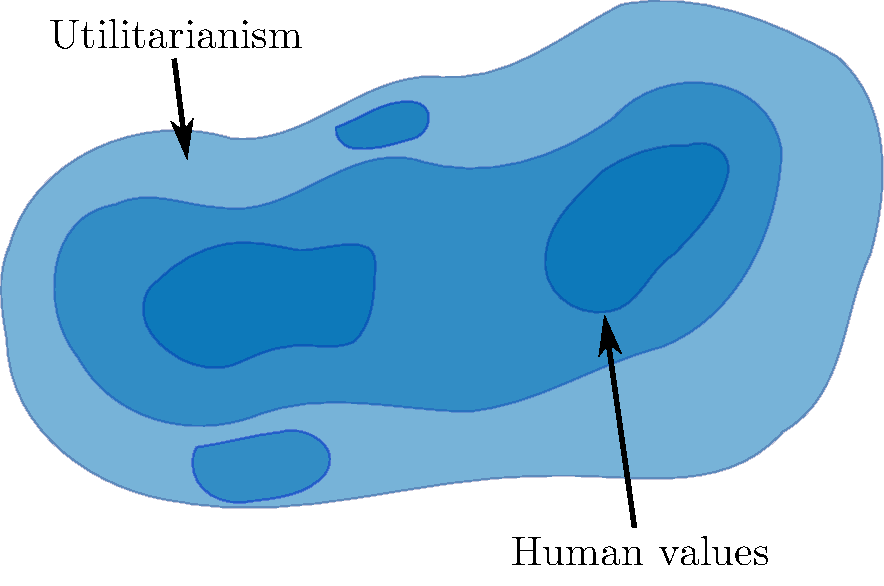
\includegraphics[width=3.26772in]{figs/map-of-value-space-compact}
    \caption{A map of a part of value space under the assumption that extant values occupy a
    relatively compact part of value space.}
    \label{map-of-value-space-compact}
\end{figure}

In this map, darker areas represent value systems with many agents and
lighter areas indicate value systems with fewer agents. If value space
looks more like this map than our previous one, then it is easier to
make ``guesses into value space'' to help superrational collaborators.
As long as one is roughly aiming at the right part of value space, small
errors just mean that one benefits slightly different superrationalists
than intended.

Only a few maps of humanity's value space have been created, the
best-known of which is probably the
\href{https://en.wikipedia.org/wiki/Inglehart\%E2\%80\%93Welzel_cultural_map_of_the_world}{\emph{Inglehart-Welzel
cultural map of the world}}. I would nonetheless wager some guesses as
to how more fine-grained maps of values would look like: on any
individual planet, there are clusters formed by major religions,
nations, political camps, and other cultural groups. For example, there
are many people who hold many of the moral views of the Quran and many
who hold many of the moral views of the Bible, but presumably much fewer
who defend a mix of the two. Nonetheless, the space between the clusters
is not completely ``uninhabited''. Furthermore, the existence of these
clusters seems to be partly arbitrary, a mere result of the way that
different ideas were packaged together historically.
\href{https://en.wikipedia.org/wiki/Path_dependence}{\emph{If things had
gone slightly differently}}, as they doubtlessly do in other parts of
the multiverse, the authors of the Bible may have written that it is
mandatory to fast during the month of Ramadan, thus filling a spot in
value space with life that is only sparsely inhabited on Earth. If the
multiverse is large enough, all these possible variations of values are
realized somewhere and probably no less common than the two religion
clusters on Earth.

One last difference between the way we extract values from other
superrational cooperators and the way AIs might receive their values
from humans is, of course, that the former involves no direct contact.
Section \ref{the-values-of-our-superrational-collaborators-in-the-multiverse} will address ways of
circumventing this problem in order to identify the values of agents elsewhere in the multiverse.

\subsubsection{The ability to help
others}\label{the-ability-to-help-others}

In some cases, it will not be in our power to help other value systems
\emph{at all}. Since any will to cooperate with these agents cannot
possibly be action-guiding, we do not have to help them. Other agents in
the universe may have other resources available to them and thus choose
to behave in a friendly way toward these values. If, on the other hand,
agents know that nobody else can help them to achieve their goals,
multiverse-wide superrational cooperation (in particular, any version of
it in which they just give resources away) becomes less attractive to
them.

One example of a value system that we cannot help is the following
version of
\href{https://en.wikipedia.org/wiki/Speciesism}{\emph{speciesism}} (that
may or may not be a
\href{https://en.wikipedia.org/wiki/Straw_man}{\emph{straw man}}):

\begin{quote}
\textbf{The Namuh-centrists.} One day, scientists inform you about a
highly intelligent species of extraterrestrials known as ``Namuhs''.
Like us, the Namuhs have built a flourishing civilization with art,
trade, science, language, humor, philosophy (including advanced decision
theory research), and so on. However, the Namuhs do not live in our
universe, but in a distant part of the multiverse, completely
inaccessible to us. In fact, they could not even exist in our part of
the multiverse, as their bodies require slightly different laws of
physics to function. Knowing about superrational cooperation, you hasten
to ask whether they have thought about problems analogous to
\href{https://en.wikipedia.org/wiki/Newcomb\%27s_paradox}{\emph{Newcomb's
problem}} and the donation games between similar agents. A trustworthy
scientist explains that their minds are indeed prone to thinking about
such topics -- much more so than those of humans, in fact!
Understandably thrilled, you ask what values the Namuhs have, and
specifically what values are held by those who have thought about
acausal cooperation. The scientist then informs you that all Namuhs are
very narrowly focused on their own species. They are Namuh-centrists who
do not care one bit about anything that does not involve fellow Namuhs.
For example, they shrug at the thought of non-Namuh
\href{https://foundational-research.org/the-case-for-suffering-focused-ethics/}{\emph{suffering}},
the flourishing of non-Namuh civilizations, or non-Namuh well-being. In
fact, they are so strict that they do not even care about simulated
Namuhs or other approximations.
\end{quote}

Learning about their values, you may be disappointed. There is nothing
that you can do to help them and it is therefore irrelevant whether they
use a decision theory similar to yours or not.

I should point out that the speciesism endorsed by the imaginary Namuhs
is very rigid and more narrow than most other views that we would
usually classify as speciesist. Far from caring only about their own
species, most people seem to care about the welfare of non-human animals
to at least some degree, usually while privileging some species (like
cats and dogs) over others (like pigs and cows). Such views classify as
speciesist, but nevertheless allow for superrational cooperation. Other
views do not value humans over other animals for their species
membership per se, but instead privilege other characteristics that
(allegedly) only humans (and sometimes a few other species) possess. A
\href{https://en.wikipedia.org/wiki/Animal_consciousness\#Philosophical_background}{\emph{common
variant}} of this holds\footnote{Note that some authors are skeptical to
  there being any fact of the matter in questioning whether some being
  is conscious or not. Instead, they view terms like ``consciousness''
  and ``sentience'' as definitional categories or expressions of
  particular values. See, e.g., \parencite{Dennett1991-es}
  and Brian Tomasik's
  \href{http://reducing-suffering.org/dissolving-confusion-about-consciousness/}{\emph{Dissolving
  Confusion about Consciousness}}.} that only members of very few
species are conscious. Humans are one of them, but, according to such
views, they otherwise do not deserve any special moral status. Given the
implications of this view, proponents are sometimes (and often
incorrectly) branded as speciesist. If the Namuhs were to hold such a
view, and humans (or other earthly species) meet their criteria for
consciousness, then our decisions \emph{can} be beneficial or
detrimental to the Namuhs' preference fulfillment. A similar reasoning
applies to the
\href{https://en.wikipedia.org/wiki/Animal_consciousness\#Language}{\emph{possession
of language}}, \href{https://en.wikipedia.org/wiki/Free_will}{\emph{free
will}},
\href{https://en.wikipedia.org/wiki/Animal_consciousness\#Mirror_test}{\emph{the
ability to pass the mirror test}} or other (potentially) strict but
non-speciesist restrictions to one's set of morally relevant agents.

There are other reasons why we might be (practically) unable to help
other agents. For example, helping an agent could require some set of
specialized abilities that they themselves developed based on their
value systems. Consider the following example:

\begin{quote}
\textbf{The Advanced math maximizers.} One day, you learn that out there
in the multiverse, there are civilizations made up entirely of
mathematicians whose primary concern is maximizing mathematical
knowledge. They don't care about the number of established truths or
proofs per se, but rather value pieces of knowledge based on their
novelty or interestingness, possibly resembling the way earthly
mathematicians often prioritize their research. For instance, the
mathematicians place a very high value on a proof or disproof of the
\href{https://en.wikipedia.org/wiki/Riemann_hypothesis}{\emph{Riemann
hypothesis}}, whereas mundane factoids like the three-billionth digit of
\(\pi\) have very little value in comparison. Moreover, once a fact
becomes known to at least one of the mathematicians, reproducing that
same piece of information elsewhere in the multiverse creates no
additional value for them. (We assume that the universe is finite --
otherwise every piece of knowledge may be known to some
\href{https://en.wikipedia.org/wiki/Boltzmann_brain}{\emph{Boltzmann
brain}}.) While they are not particularly skilled at anything else,
their strong intrinsic motivation and dedication has made them into
truly excellent mathematicians, unrivalled by anyone across the
multiverse.
\end{quote}

It is not easy to benefit the advanced math maximizers. We do not know
what knowledge they already possess, and given their level of skill, we
should assume that they will come up with most interesting pieces of
mathematical knowledge that we could devise on our own. The math
maximizers are thus so capable of maximizing their own utility function
that there is little we could do to assist them (cf. section
\ref{gains-through-specialization-and-comparative-advantages}).

\hypertarget{zero-sum-and-below-zero-sum-tradeoffs-on-resources}{\subsubsection{Zero-sum
and ``below-zero-sum'' tradeoffs on
resources}\label{zero-sum-and-below-zero-sum-tradeoffs-on-resources}}

Not all interactions between agents allow for cooperation. Specifically,
there is no way or reason to cooperate in
\href{https://en.wikipedia.org/wiki/Zero-sum_game}{\emph{zero-sum}}
\href{https://en.wikipedia.org/wiki/Zero-sum_game}{g}a\href{https://en.wikipedia.org/wiki/Zero-sum_game}{m}e\href{https://en.wikipedia.org/wiki/Zero-sum_game}{s},
i.e. ones in which the overall payoff is always the same. Consider the
following example:

\begin{quote}
\textbf{The Maximizer Monarchs.} Imagine a multiverse consisting of two
universes. One is ruled by a queen whose only drive it is to create as
many paperclips as possible. The other universe is ruled by a king who
only cares about producing as many staples as possible. Each
stationery-maximizing monarch knows that the other exists and that they
both use the same decision algorithms. They each have one hundred tons
of steel at their disposal. What should they do with it?
\end{quote}

Assuming that staples (specifically the kind of staples that the queen
cares about) cannot be built out of paperclips or vice versa, this
interaction is zero-sum. Every bit of material that one of them uses for
the benefit of the other is an equivalent loss to themselves\footnote{If
  we normalize their utility function, both assign the same utility to a
  situation in which all the multiverse's metal is transformed into
  their favorite office supply. This also means that they assign the
  same utility to any other other fixed amount of metal being
  transformed into paperclips.}. Thus, no form of cooperation between
the two is beneficial.

As the reader may suspect, zero-sum interactions are rare. We should
expect that any given resource is better suited to achieving one goal
than another and so trade can arise from allocating resources based on
what value systems benefit most from them. Analogously, value systems
care more about certain situations than others. Furthermore, whereas it
may not be possible to combine a paperclip and a staple, many goals are
compatible with each other. For example, a society's citizens can at the
same time be happy and virtuous.

\hypertarget{gains-through-specialization-and-comparative-advantages}{\paragraph{Gains
through specialization and comparative
advantages}\label{gains-through-specialization-and-comparative-advantages}}

At times, trying to achieve multiple goals at once is not just pointless
-- it can actually be worse than having each agent focus on one,
typically their own, goal. To see how, let us revisit The Maximizer
Monarchs of the previous section:

\begin{quote}
\textbf{The Ever-improving Maximizer Monarchs.} Like The Maximizer
Monarchs, but this time, the efficiency at which each agent can produce
paperclips or staples grows monotonically with the produced quantity.
Again, each monarch wields one hundred tons of steel.
\end{quote}

Without delving into mathematical details, it is best (in terms of
overall number of paperclips/staples produced) if each of the two
specializes in one kind of stationery. In particular, there are no gains
from compromise over each monarch maximizing only for their own goals.

There may also be
\href{https://en.wikipedia.org/wiki/Comparative_advantage}{\emph{comparative
advantages}} from the outset. Based on their respective motivation and
prior experience, the queen may already excel at producing paperclips,
while the king may be better at producing staples. Another important
source of comparative advantages is unequal knowledge about different
value systems. For example, if the queen does not know exactly what the
king cares about, then she will be worse at benefitting him. Similarly,
our knowledge of what other humans care about is much more precise than
our knowledge of what agents elsewhere in the multiverse care about.

The fact that specialization and division of labor play such a crucial
role in the economy suggests that superrationalists will also tend to
focus on a single goal rather than maximizing for multiple things at
once. However, I think that this will not be the case, at least in our
present situation. The primary reason is that the instrumental goals of
agents with different moral values are often the same. For example, no
matter the direction into which we would like to drive society, we will
try to acquire money and political influence. These resources are often
generic, such that when they are acquired with one goal in mind, they
can also be employed in pursuit of another. As an example, consider how
Donald Trump maximized his personal monetary wealth for a long time, yet
his resulting fame and money nevertheless enabled him to become
president of the US, which in turn allows him to achieve all kinds of
goals. The fact that instrumental goals tend to converge suggests that
superrationalists in the multiverse rarely have a strong comparative
advantage at achieving their own goals.

If comparative advantages are not strongly aligned with goals,
specialization can produce gains as well. For example, imagine a number
of superrational agents, each of whom would like to maximize many
different things separately, e.g., knowledge, fun, happiness and
technology. Here, a no-compromise outcome -- i.e. one wherein each agent
only maximizes their utility function in their own universe -- might be
worse than a potential division of labor with one agent focusing on
generating knowledge, another one focusing on fun, and so forth.

\hypertarget{what-values}{\subsection{What values?}\label{what-values}}

To help other agents, one at some point needs to have some workable
model of their preferences. In general, it is difficult to extract
preferences from a given agent
\href{http://lesswrong.com/lw/h45/we_dont_have_a_utility_function/}{\emph{if}}
the agent is not
\href{https://en.wikipedia.org/wiki/Von_Neumann\%E2\%80\%93Morgenstern_utility_theorem}{\emph{von
Neumann-Morgenstern (vNM) rational}} and cannot state her goal
explicitly. Humans surely
\href{https://en.wikipedia.org/wiki/Cognitive_bias}{\emph{are not}}
vNM-rational. Additionally, moral judgments are usually seen as being
inaccessible to us in their complete form (see footnote
\ref{we-do-not-know-our-utility-function}) and as emerging from the whole
brain rather than exclusively from, say, the anterior cingulate cortex.
This makes sense from an evolutionary point of view. Preferences are
tools for increasing the fitness of an organism, and there is no reason
to assume that such tools would be any more open to scrutiny by the
organism than, say, the detailed inner workings of the digestive system.
In addition, while most organisms have rudimentary mechanisms for
avoiding harm and seeking food and reproduction, holding grudges -- i.e.
a preference for retaliation -- is only adaptive in non-solitary
organisms with sufficiently good memory and recognition to correctly
identify transgressors. In the evolutionary process, different values
thus evolve separately and are unlikely to form a coherent whole (cf.
\cite{Dennett1991-es,Kurzban2012-vt}).

Thus, even if we had a complete model of our superrational
collaborators, it would nevertheless be difficult to extract clear-cut
values from them. In the absence of such exact models, it makes little
sense to for us to discuss the technical details of relevant preference
extraction algorithms\footnote{Examples are described in
\cite{Hansson2012-um,Varian2006-vw,Von_Neumann1953-mc,Ng2000-xw,Oesterheld2016-bh}. Also consider Brian Tomasik's \href{http://reducing-suffering.org/interpret-physical-system-mind/}{\emph{How to Interpret a Physical System as a Mind}}.}.
We will, however, still
need to think about informal ways of inferring preferences from a model
of a superrational collaborator.

\subsubsection{Idealization}\label{idealization}

One dimension along which preference extraction algorithms vary is the
extent to which they idealize values. Consider the following example of
preference idealization (adapted from
\href{https://casparoesterheld.com/2017/01/18/is-it-a-bias-or-just-a-preference-an-interesting-issue-in-preference-idealization/}{\emph{a
recent blog post of mine}}): Steve holds a glass of transparent liquid
in his hand. A woman walks by, says that she is very thirsty and that
she would like to drink from Steve's glass. What she does not know,
however, is that the water in the glass is (for some unspecified reason)
poisoned. Should Steve allow her to drink? Most people would say he
should not. While she does want to drink from the glass, her desire
would probably disappear upon learning of its content. Therefore, one
might say that her \emph{object-level} or \emph{stated} preference is to
drink from the glass, while her \emph{idealized} preference would be not
to drink from it.

Similar questions apply to ethical preferences. For example, most people
find meat consumption acceptable on the object-level, but are simply
unaware of information about the world that could change their minds,
e.g., knowledge about the similarities between human and animal minds or
the
\href{https://en.wikipedia.org/wiki/Animal_welfare\#Farm_animals}{\emph{conditions
in factory farms}} and
\href{https://en.wikipedia.org/wiki/Slaughterhouse\#Animal_welfare_concerns}{\emph{slaughterhouses}}.
Perhaps these
\href{http://www.telegraph.co.uk/food-and-drink/news/number-of-vegans-in-britain-rises-by-360-in-10-years/}{\emph
    {people's idealized preferences}} favor vegetarianism? If we reduce meat consumption, should we
count it as beneficial to people who approve of eating meat, but who could be convinced
otherwise? Should we, in other words, idealize our collaborators' values when taking them into
account in this universe?

Besides gaining more information about the world, people's preferences
may also change upon engaging with \emph{moral} arguments (e.g., the
\href{http://plato.stanford.edu/entries/original-position/}{\emph{original
position}} or the
\href{https://en.wikipedia.org/wiki/Famine,_Affluence,_and_Morality}{\emph{drowning
child argument}}). Even though such arguments do not provide new facts,
they may invoke trains of thought that lead people to change their moral
position. Should we also idealize preferences based on such moral
arguments?

At least idealization based on moral argument can cause trouble. For
one, some moral arguments can be viewed as potentially illegitimate
``tricks'' for persuading people to adopt undesired positions\footnote{One
  class of such tricks is described in my blog post
  \href{https://casparoesterheld.com/2015/12/06/cheating-at-thought-experiments/}{\emph{Cheating
  at thought experiments}}.}. An extreme example of this could be some
moral or religious scripture that hypnotizes and brainwashes the reader.
Surely, nobody would want other superrational collaborators to apply
such a treacherous ``idealization procedure''.

\href{http://www.philosophyexperiments.com/sedan/Default5.aspx}{\emph{Order
effects}} constitute another problem in using moral arguments to
idealize preferences. Depending on the order in which we present someone
with moral arguments, they may lock into a position and resist further
arguments. If someone's moral views allow for more than one such lock-in
they may not be uniquely idealizable. A recent study by
Schwitzgebel and Cushman shows that even philosophers
exhibit order effects when considering thought experiments~\parencite{Schwitzgebel2012-vh}.

In general, we may view agents as having (meta-)preferences regarding
idealization. These determine how exactly they would like to have their
values idealized. We should then abide by respective agent's
preferences, since we can then expect others to idealize our values in
the way that we want them to be idealized. Unfortunately, this solves
the problem only theoretically. In practice, finding out what
idealization procedures other superrationalists would approve seems very
difficult.\footnote{In
  \href{https://agentfoundations.org/item?id=1492}{\emph{Divergent
  preferences and meta-preferences}}, Stuart Armstrong makes a few
  points that are closely related to the preceding three paragraphs.}

For more thoughts on preference idealization, the reader may consult any
of the following:
\cite{Yudkowsky2004-fz,Tomasik2016-cb,Grill2015-wk,Muehlhauser2012-ib};
the
\href{https://www.utilitarianism.com/nu/nufaq.html}{\emph{Negative
Utilitarianism FAQ,} especially}
\href{https://www.utilitarianism.com/nu/nufaq.html\#2.1}{\emph{section
2.1}}; and my blog post entitled
\href{https://casparoesterheld.com/2017/01/18/is-it-a-bias-or-just-a-preference-an-interesting-issue-in-preference-idealization/}{\emph{Is
it a bias or just a preference? An interesting issue in preference
idealization}}, in which I discuss the specific issue of removing
cognitive biases from preferences.\footnote{Habermas' discourse ethics
  is also worth mentioning. Alas, the best discussion of its main ideas
  that I am aware of -- ch. 5 of Norbert Hoerster's \emph{Wie lässt sich
  Moral begründen?} -- is currently only available in German.}

\paragraph{Beware motivated
idealization}\label{beware-motivated-idealization}

One potential pitfall of idealizing another agent's values is that it
might bias the result toward one's own moral views if one is not
careful. After all, you will be more familiar with the arguments and
thought processes that favor your own position, and they will seem more
convincing to you than the arguments you know in favor of other
positions (if you knew of similarly strong arguments in favor of other
positions, there is a good chance you would have adopted them already).
Such a process of legitimizing what we already want to do via
superrationality-based reasoning could be nicknamed
``superrationalizing''. For instance, I might be tempted to think that
supporters of
\href{https://en.wikipedia.org/wiki/Deep_ecology}{\emph{deep ecology}}
and (non-anthropocentric)
\href{https://en.wikipedia.org/wiki/Environmentalism}{\emph{environmentalism}}
would, if they were rational, update their views significantly upon
learning about Darwinian evolution and
\href{https://foundational-research.org/the-importance-of-wild-animal-suffering/}{\emph{wild
animal suffering}}. I may even presume that deep ecologists would
support intervention in nature or even
\href{http://reducing-suffering.org/habitat-destruction-not-preservation-generally-reduces-wild-animal-suffering/}{\emph{habitat
destruction}} under idealization! While I do indeed think that many
people's judgment of nature and preservation would change significantly
upon understanding the above topics\footnote{On the other hand, many (if
  not most) biologists seem to care about conservation -- popular
  biology textbooks like \emph{Campbell Biology} \parencite{Urry2016-ey}
  and \emph{Life: The Science of Biology} \parencite{Sadava2012-er}
  cover and seem to endorse
  \href{https://en.wikipedia.org/wiki/Conservation_biology}{\emph{conservation
  biology}}. There are various counter-considerations, though. For
  example, a prior concern for the environment may be a strong motivator
  for many to study biology in the first place. Perhaps many also did
  not think about the moral value of nature all that systematically, and
  instead base their views on more subjectively relevant metrics like
  novelty or aesthetics. From what I can tell, neither \emph{Campbell
  Biology} nor \emph{Life} cover wild animal suffering at all in their
  textbooks.}, I am worried about what such an aggressive stance on
idealization tells me about the way other agents might go about
idealizing values. For instance, when idealizing \emph{my} values,
environmentalists might reason that I just never thought enough about
the beauty of nature. ``If only this Caspar guy had taken the time to
really contemplate the natural world in all its magnificent complexity,
he would not think of nature as a tragedy, no matter how
`\href{https://en.wikipedia.org/wiki/In_Memoriam_A.H.H.}{\emph{red in
tooth and claw}}'
\href{https://en.wikipedia.org/wiki/In_Memoriam_A.H.H.}{i}t
m\href{https://en.wikipedia.org/wiki/In_Memoriam_A.H.H.}{a}y be.''
Consequently, they might conclude that it is in my idealized interest if
they lobby for leaving nature untouched or even spread it to other
planets. I would not want others to idealize my values in such a way.
While it may be true that a sufficient amount of time spent enjoying
beautiful landscapes could convince me that nature is beautiful, I might
not view that as a legitimate idealization procedure, as it merely
reinforces conservationist arguments rather than offering new arguments
or some form of balanced view.

An example of a more obviously flawed extrapolation process is that of a
mother reasoning that everyone's idealized values would be to prefer her
son over all other children. After all, if they only spent enough time
with him (just as she did), they would surely prioritize his well-being
over that of other children! Once again, the respective idealization
process seems unduly biased towards a certain position and will thus be
rejected by most agents' meta-preferences.

\hypertarget{values-and-distance}{\subsubsection{Values and
distance}\label{values-and-distance}}

People care about things differently depending on whether they happen
nearby or far away in space and time. For example, while many liberals
and quite a few conservatives politically favor legalizing cannabis, I
expect that many of them would nevertheless feel mildly annoyed or
uncomfortable if their best friend, spouse, or daughter were to start
smoking it on a regular basis. For brevity, I will use the term
\emph{near values} for the part of our values that are about near things
and \emph{far values} for the part that is concerned with distant
things. Both in the ancestral environment and today, most people operate
primarily on their near values (with one notable exception being
politics). In the context of superrationality, however, we are only
interested in far values. Most other superrationalists are so far away
from us that our values pertaining to their worlds fall under our far
values. Hence, we want ETs to consider only our far values, which in
turn means we should only consider the ETs' far values as well. That is,
we do not need to know how they want their friends to treat each other,
how they feel about drug use in their own social circles, and so forth.
(Some think that the discrepancy between near and far values should
disappear under idealization; we will discuss this below.)

According to
\href{https://en.wikipedia.org/wiki/Construal_level_theory}{\emph{construal
level theory}}, the difference between near and far values mainly
results from the difference between two kinds of thinking or
\emph{construal}: concrete (or low) and abstract (or high) levels of
construal. Which level of construal is applied mainly depends on the
psychological distance to an event, i.e. the combined temporal, spatial,
social and ``hypothetical'' (near = likely, far = unlikely) distance.
People tend to construe psychologically near events concretely and
psychologically far events abstractly. A recent summary of construal
level theory is given by
\href{http://www.psych.nyu.edu/trope/Trope_Liberman_2010.pdf}{\emph{Trope
and Liberman (2010)}}.

The mapping between levels of construal and psychological distance is
imperfect. We sometimes think about psychologically distant things
concretely, such as when watching a science-fiction movie, and about
psychologically near things abstractly. Nevertheless, the mapping is
useful. While there is little theoretical and empirical research on how
people (and other evolved creatures of human-level intelligence) think
and care about alien civilizations, there is some research on how people
generally care about other psychologically distant and abstractly
construed things. According to construal level theory, the abstract mode
of thinking is similar regardless of the kind of psychological distance
that is involved. Thus, we can use general research about abstract
construal values to at least inform our first tentative guesses about
values in the particular case of caring about distant civilizations.

We have some reasons to expect construal level theory to generalize to
other evolved beings. According to Trope and Liberman (2010, section
III, subsection ``Discussion''),

\begin{quote}
High-level construals and low-level construals serve different cognitive
functions. High-level construals have evolved to represent distal
objects because, with distance, one needs to conserve the essential,
invariant properties of the referent object. In contrast, low-level
construals preserve the object in minute detail for immediate use.
\end{quote}

The fact that abstract and concrete construals solve different problems
suggests that they evolved separately. Indeed, low-level construals
probably evolved earlier. Whereas processing one's immediate
surroundings and short-term goals is necessary for any animal to
survive, many can get by without processing psychologically distant
things. Some of the feats achieved by civilization-forming species, on
the other hand, require abstract thinking. In the conclusion of their
paper, Trope and Liberman (2010) write:

\begin{quote}
The turning points of human evolution include developing tools, which
required planning for the future; making function-specific tools, which
required considering hypothetical alternatives; developing
consciousness, which enabled the recognition of distance and perspective
taking; developing language, which enabled forming larger and more
complex social groups and relations; and domestication of animals and
plants, which required an extended temporal perspective
\href{http://web.missouri.edu/~gearyd/Flinnetal2005.pdf}{\emph{(Flinn,
Geary, \& Ward, 2005)}}. Human history is associated with expanding
horizons: traversing greater spatial distances (e.g., discovering new
continents, space travel), forming larger social groups (families vs.
cities vs. states vs. global institutions), planning and investing in
the more distant future, and reaching farther back into the past.
\end{quote}

In sum, I see some good reasons to expect that construal level theory
applies to many other evolved species of human-level
intelligence.\footnote{The presented argument resembles the general
  argument for
  \href{https://en.wikipedia.org/wiki/Modularity_of_mind}{\emph{modularity}}
  in evolutionary psychology (see, e.g.,
  \href{http://citeseerx.ist.psu.edu/viewdoc/download?doi=10.1.1.140.7758\&rep=rep1\&type=pdf}{\emph{Cosmides
  and Tooby 1994}}).} It thus matters whether we optimize for others'
near or far values.

Interestingly, we may also see the difference between different
construals and thus near and far values as a cognitive bias that would
disappear upon reflection, and that we should correct for in preference
idealization. This may well be the case, but it is unclear which of the
two views is more ``correct'' about ethics. One may argue that only
thinking about concrete events can yield actual moral judgments, while
abstract thinking may result in imagining a situation inaccurately or
not at all and thus being unable to assess it correctly. Moreover, we
tend to have weaker attitudes in general toward distant things than
towards close things,\footnote{For example, people
  \href{https://en.wikipedia.org/wiki/Time_preference}{\emph{prefer}} to
  receive money immediately rather than in the far future. They are
  \href{https://en.wikipedia.org/wiki/Risk_aversion}{\emph{risk averse}}
  and, of course, care more about socially close individuals. They are
  also more relativist when judging the acts of extraterrestrials and
  people from other cultures \parencite{Sarkissian2011-be}.}
and this also seems to apply to moral weight assignment.\footnote{For
  example, thinking about a concrete, identifiable goal or benefactee
  seems to be associated with feeling
  \href{https://en.wikipedia.org/wiki/Warm-glow_giving}{\emph{happier
  from donating money}}
  (\href{https://dash.harvard.edu/bitstream/handle/1/12534961/rudd,aaker,norton_getting-the-most-out-of-giving.pdf?sequence=3}{\emph{Rudd
  et al. 2014}}). People are more motivated by (concrete)
  \href{https://en.wikipedia.org/wiki/Identifiable_victim_effect}{\emph{identifiable
  victims}} than by (abstract) large numbers of victims, although a
  recent meta-study by Lee and Feeley shows the
  effect to be small~\parencite{Lee2016-lb}.}

Some arguments in moral philosophy evoke concrete construals (e.g.,
\href{https://en.wikipedia.org/wiki/Trolley_problem\#The_fat_man}{\emph{the
fat man trolley problem}} or the
\href{https://en.wikipedia.org/wiki/Famine,_Affluence,_and_Morality}{\emph{drowning
child argument}}) and some evoke abstract construals (e.g., the
\href{https://en.wikipedia.org/wiki/Original_position}{\emph{original
position}} or many of the examples from my blog post
\href{https://casparoesterheld.com/2015/12/06/cheating-at-thought-experiments/}{\emph{Cheating
at thought experiments}})\footnote{Many arguments also present a
  conflict between abstract and concrete thinking. For example, the
  \href{https://en.wikipedia.org/wiki/Mere_addition_paradox}{\emph{repugnant
  conclusion}} can be seen as a clash of the evaluation by the concrete
  welfare of the
  \href{https://en.wikipedia.org/wiki/Identifiable_victim_effect}{\emph{identifiable
  victim}} or
  \href{https://en.wikipedia.org/wiki/Peak\%E2\%80\%93end_rule}{\emph{representative
  moment}} and the abstract evaluation by the aggregate welfare.}. Both
classes contain arguments that I find useful and legitimate. This
suggests that neither of the two is morally superior across the board.

Trope and Liberman (2010, section VI) describe several experiments
wherein high-level construals seem to capture the participants' values,
whereas low construals led people to give more weight to ``local''
circumstances (such as social pressure and lack of self-control) (cf.
Trope and Liberman 2010, section VII, subsection ``Affect''). In high
levels of construal, people tend to judge consequences more by their
desirability than their feasibility, and thus assign more weight to
moral views. More recent studies like those of Torelli and Kaikati 
\parencite{Torelli2009-mw} and Agerström and Björklund~
\parencite{Agerstrom2013-ep} have corroborated this result.
However, it
\href{http://www.overcomingbias.com/2010/05/far-is-hypocritical.html}{\emph{could}}
also be interpreted as an indication that abstract thinking makes people
more hypocritical.

\href{http://minerva.union.edu/bizerg/readings230/wk04.pdf}{\emph{Yang,
Preston and Hernandez (2012)}} summarize further evidence in favor of
giving more weight to high-construal judgments:

\begin{quote}
High-level construal is associated with {[}...{]} an analytical,
critical-thinking mind-set
\href{http://citeseerx.ist.psu.edu/viewdoc/download?doi=10.1.1.186.6465\&rep=rep1\&type=pdf}{\emph{(Torelli
and Kaikati, 2009)}}. For example, people at a high level of construal
are {[}...{]} more comfortable with messages that convey mixed emotions
\href{http://www.bm.ust.hk/mark/staff/Jiewen/Jiewen\%20JCR-Oct\%202010.pdf}{\emph{(Hong
and Lee, 2010)}}, suggesting greater cognitive flexibility. Indeed,
previous literature showed that when an object is distanced from the
self, individuals are less likely to be ``trapped'' in their own
preconception or knee-jerk reactions
\href{https://uwaterloo.ca/wisdom-and-culture-lab/sites/ca.wisdom-and-culture-lab/files/uploads/files/kross_grossmann_jepg_2012.pdf}{\emph{(Kross
and Grossmann, 2012)}}. Moreover, high levels of construal may enhance
perspective taking toward others whose interests conflict with one's
own.
\end{quote}

That said, abstract thinking is not without its systematic failure
modes. It is, for instance, associated with
\href{https://en.wikipedia.org/wiki/Overconfidence_effect}{\emph{overconfidence}}
and the \href{https://www.edge.org/response-detail/27117}{\emph{illusion
of explanatory depth}} \parencite{Alter2010-lu}.

Further thoughts on the topic are given by Samuel Hammond in
\href{http://abstractminutiae.com/post/85550239565/how-to-conceptualize-morality-near-vs-far}{\emph{How
to Conceptualize Morality: Near vs Far}}. In any case, we should keep
in mind that idealizing away the difference between near and far values
may be inconsistent with many agents' meta-preferences.

\subsubsection{Different kinds of
preferences}\label{different-kinds-of-preferences}

People often report that preferences in different domains feel
qualitatively different from one another. For instance, it is common to
distinguish moral preferences from other preferences. My preference for
world peace over war is a moral one, for instance, but my preference for
bananas over carrots is not. This line between moral and non-moral
values is often blurry. For example, it is unclear whether wanting
revenge or a cancer victim's desire to focus altruistic efforts on
cancer research are moral preferences. I think such a distinction can be
drawn even among far values. For example, my preferences for beings in
other parts of the multiverse to be happy rather than to suffer is a
moral one, but I would not view my preference for these civilizations to
be fascinating, fun, or otherwise beautiful to my eyes (in the way that
advanced civilizations in science fiction movies are) as a moral
preference. Others might disagree, but that dispute is not worth
exploring in this paper (indeed, I suspect it may be a largely verbal
one). Potential criteria for this distinction between moral and other
preferences may be that moral preferences are those we want others to
share or that are somehow universal.

Another distinction could be one based on a
\href{https://en.wikipedia.org/wiki/Dual_process_theory_(moral_psychology)}{\emph{dual-process
theory of morality}} (see Greene 2013, part II for an overview and
references to the literature). Or consider
\parencite{noauthor_undated-wg}, who propose that ``what we
call human values can be decomposed into 1) mammalian values, 2) human
cognition, and 3) several millennia of human social and cultural
evolution.''

I do not think such distinctions are necessary when cooperating
superrationally. Instead, we should focus on all preferences that are
action-guiding to the respective agent (if this is not included in the
term ``preference'' anyway\footnote{Many definitions of preferences are
  based on choice. (TODOLaTeX: refer to the other footnote where I list
  ways in which preferences are defined) Some examples where preferences
  may not be what our choices reveal include:

  \begin{quote}
  \href{https://en.wikipedia.org/wiki/Akrasia}{\emph{akrasia}} and lack
  of willpower, as it manifests itself in
  \href{https://en.wikipedia.org/wiki/Procrastination}{\emph{procrastination}}
  and inability to adhere to exercise routines and healthy diets;
  \end{quote}

  \begin{quote}
  preferences about fiction, as people often care deeply about how a
  story ends
  \href{http://briantomasik.com/collection-quick-observations/\#Taking_fiction_seriously}{\emph{but
  usually without}} trying to lobby or coerce the authors to satisfy
  that desire
  \parencite{Radford1975-my,noauthor_undated-sw}; and
  \end{quote}

  \begin{quote}
  preferences for states of affairs that are mathematically inconsistent
  or physically impossible~\cite{Oesterheld201X}. 
  %(Oesterheld, unpublished TODOLaTeX)
  \end{quote}}), irrespective of whether they are ``moral'' or
``mammalian''. By definition, if I have to decide between two courses of
action and one of them better suits the preferences that guide my
actions, I will choose that one. In the case of superrationality, only
accounting for other agents' action-guiding preferences correlates with
others also taking only my action-guiding preferences into account.
Therefore, taking all action-guiding preferences into account is best
according to my action-guiding preferences. Hence, we should only take
steps to fulfill the action-guiding preferences of other superrational
collaborators, ignoring any other preferences they might hold.

Given the above, I shall in this piece not differentiate between moral
and other far values. Instead, both terms will be used to signify our
action-guiding far values, moral or not.

\hypertarget{the-values-of-our-superrational-collaborators-in-the-multiverse}{\subsection{The
values of our superrational collaborators in the
multiverse}\label{the-values-of-our-superrational-collaborators-in-the-multiverse}}

Having outlined what kinds of values we would like to know about for
multiverse-wide superrational cooperation, we can finally proceed to
discuss these values. Whereas it is not strictly necessary for us to
know about our cooperators' values right away in order to benefit them
(see section
\ref{cooperation-in-the-face-of-uncertainty-about-values}), such
knowledge is surely useful and has to be attained at some point. In
fact, one objection to multiverse-wide superrationality (MSR) that many
people have brought up in private conversation is that given our
uncertainty about other value systems in the multiverse we should focus
solely on our own values (also see section
\ref{objection-based-on-uncertainty-about-the-values-of-superrationalists-in-the-multiverse}). As readers may suspect, a comprehensive discussion of
this topic is beyond the scope of the present paper. However, we will
give an overview of how we (or future superrationalists) can gain
knowledge about the values of our collaborators elsewhere in the
multiverse. Besides guiding future research, this overview will also
demonstrate that we can learn anything about their values in the first
place.

It seems as though there are two main ways of assessing the values of
other agents in the multiverse. The first involves empirical research
into the values of superrational cooperators on Earth. Because the
sample size is so small, we may also look at humans in general, under
the assumption that the values of superrationalists resemble the values
of their native civilization. It may be that the values of
superrationalists differ from those of other agents in systematic and
predictable ways. General human values may thus yield some useful
insights about the values of superrationalists. That said, it may be
that only a small fraction of superrationalists in the multiverse are
human-like. For example, it could be that most other superrationalists
are artificial intelligences and
\href{https://en.wikipedia.org/wiki/Mind_uploading}{\emph{whole-brain
emulations}}. It could also be that many other evolved agents are very
different from us.

The other approach involves understanding the processes that generate
and select the values of agents in the multiverse, such as biological
and cultural evolution, the transition to superintelligent AIs, etc.,
and extrapolating them into workable predictions about the preferences
of agents on other planets. In principle, this approach is sufficient
for gathering a good map of the values of civilizations throughout the
multiverse. In practice, however, it is probably very difficult to
accurately predict how these processes play out. A combination of both
approaches might be easier to work with. We can begin with human values
as a baseline and inspiration for what kinds of moral attitudes may
exist, and then review whether the processes of biological and cultural
evolution systematically favor these attitudes. This would enable us to
find out whether they are coincidental and hence rare in the multiverse,
or necessary and thus common. At the same time, we will of course need
to avoid being biased toward human values, making sure not to drift off
into telling
\href{https://en.wikipedia.org/wiki/Just-so_story}{\emph{just-so
stories}} about why some human practices and values might be universal
among evolved agents of human intelligence
\parencite{Buss2015-kp}. Theoretically, we or future
superrationalists need to find some way of coming up with new moral
values, i.e. ones that we do not observe on Earth. Based on a model of
the values of evolved agents we can then think about the values of these
agents' descendants (whole brain emulations, superintelligent AIs).

Assessing the action-guiding, consequentialist far values of agents in
the multiverse could be a scientific (sub-)discipline in its own right.
That being said, I do not expect there to be a ``Journal on
Extraterrestrial Value Systems'' to materialize anytime soon. Untestable
speculation about ETs does not inspire academic respectability. In
researching this paper, I did not find much prior work on any aspect of
the values of evolved agents in the multiverse, which in turn makes me
less than hopeful that the more specific issues pertaining to
multiverse-wide superrational compromise will be picked up by other
researchers out of curiosity. Hence, superrationalists will probably
need to think about ET values themselves.

\subsubsection{On the far values of humans and human superrational
cooperators}\label{on-the-far-values-of-humans-and-human-superrational-cooperators}

We will now explore what superrational humans might care about in
distant civilizations. Unfortunately, our sample of these people is
small, and
\href{https://en.wikipedia.org/wiki/Path_dependence}{\emph{path
dependencies}} may imply that current earthly superrationalists may not
be very representative of those elsewhere in the multiverse. We will,
therefore, also look at general human values and far values in
particular.

\hypertarget{organizing-human-values}{\paragraph{Organizing human
values}\label{organizing-human-values}}

Although most people have reliable intuitions for what other people care
about, these intuitions are hard to pin down, owing to the inherent
``messiness'' of human moral intuitions (cf.
\cite{Stewart-Williams2015-gg}, section ``Morality Is a
Mess''; \cite{Muehlhauser2012-ib}). This ``messiness''
\href{http://lesswrong.com/lw/l3/thou_art_godshatter/}{\emph{makes}}
\href{https://en.wikipedia.org/wiki/Modularity_of_mind\#Evolutionary_psychology_and_massive_modularity}{\emph{evolutionary
sense}}
(\href{http://citeseerx.ist.psu.edu/viewdoc/download?doi=10.1.1.140.7758\&rep=rep1\&type=pdf}{\emph{Cosmides
and Tooby 1994}}) and should therefore be expected from other
civilizations in the multiverse as well. To talk about human values, it
is at least helpful (if not necessary) to develop some systematic
terminology and overview of what kind of things people care about.
Luckily, we can get help from
\href{https://en.wikipedia.org/wiki/Moral_psychology}{\emph{moral
psychologists}} and others who have attempted to develop just this sort
of overview.

One example is Jonathan Haidt's and Craig Joseph's
\href{https://en.wikipedia.org/wiki/Moral_foundations_theory}{\emph{moral
foundations theory}}. It divides morality up into five foundations --
care, fairness, loyalty, authority and sanctity -- although the authors
do acknowledge that some other values (such as liberty) may deserve
foundation status as well. Haidt and his colleagues have also
\href{https://en.wikipedia.org/wiki/Moral_foundations_theory\#Political_ideology}{\emph{shown}}
that while social conservatives tend to embrace all five moral
foundations, liberals/progressives seem to focus primarily on the first
two, i.e. care and fairness.\footnote{Many other characterizations of
  the difference between liberals and conservatives have been proposed.
  For example, Robin Hanson
  \href{http://www.overcomingbias.com/2012/05/forager-vs-farmer-morality.html}{\emph{compares}}
  the
  \href{http://www.overcomingbias.com/2010/10/two-types-of-people.html}{\emph{differences
  between}} liberals and conservatives to the differences between
  foragers and farmers. Other distinctions have been proposed by
  \href{https://sl4librarian.files.wordpress.com/2017/01/sinn2016-replacing-the-moral-foundations.pdf}{\emph{Sinn
  and Hayes (2016}}) and
  \href{https://en.wikipedia.org/wiki/Moral_Politics_(book)}{\emph{Lakoff
  (1996}}).} We can thus also use the terms ``liberal'' and
``conservative'' to describe values, even though it is, of course,
uncertain whether this distinction carries the same weight in other
civilizations.

Other theories outlining what humans value include Schwartz'
\href{https://en.wikipedia.org/wiki/Theory_of_Basic_Human_Values}{\emph{Theory
of Basic Human Values}} (updated and extended by
\cite{Schwartz2012-qi}), as well as those of
\cite{Shweder1997-ge} (also see
\cite{Pinker2011-el} for a short, accessible summary).
There is also Peter Levine's
\href{http://peterlevine.ws/?p=16998}{\emph{Alternative to Moral
Foundations Theory}}, which is not formally published.

There are also some characterizations of the cultural and moral
\emph{differences} among humans. For example,
Inglehart and Welzel divide moral values into just
two factors: traditional versus secular-rational values, and survival
versus self-expression values \parencite{Inglehart2010-qr}.
\href{https://en.wikipedia.org/wiki/Geert_Hofstede}{\emph{Hofstede}}
\href{https://en.wikipedia.org/wiki/Hofstede\%27s_cultural_dimensions_theory}{\emph{recognizes}}
six cultural dimensions, and
\href{https://en.wikipedia.org/wiki/Fons_Trompenaars}{\emph{Trompenaars}}'
\href{https://en.wikipedia.org/wiki/Trompenaars\%27_model_of_national_culture_differences}{\emph{model
of national culture differences}} has seven dimensions of varying moral
relevance.

\hypertarget{human-far-values}{\paragraph{Human far
values}\label{human-far-values}}

We have seen that far values are the parts of our preferences that are
relevant to MSR (see section
\ref{values-and-distance}). There are almost no studies on how humans care about
alien civilizations. However,
\href{https://en.wikipedia.org/wiki/Construal_level_theory}{\emph{construal
level theory}} suggests that we think and thus care similarly about
different psychologically distant things. This brings us to the
question, how do people usually care about psychologically distant or
abstractly construed things?

In contrast to their concrete counterpart, values at abstract construal
levels tend to focus more on the central (as opposed to peripheral)
features of a given situation (see \cite{Trope2010-vo},
esp.
\href{http://www.psych.nyu.edu/trope/Trope_Liberman_2010.pdf\#page=12}{\emph{section
V}}). Values in abstract construal levels are therefore less fragile
(see section \ref{fragility-of-value}), which is good news for us, as this inherent stability makes
them easier to account for in our superrational cooperation. But what
are those central features?

A few studies have been conducted to find out, most notably one by
\cite{Bain2013-fc}. The authors summarize the results
in a
\href{https://spsptalks.wordpress.com/2013/07/14/the-utopias-of-everyday-people/}{\emph{blog
post}}:

\begin{quote}
In our research, we asked people to think about the effects that changes
in society today would have on society in the future (the Year 2050).
For instance, we asked people to consider what society would be like 50
years in the future if climate change was mitigated, marijuana was
legalized, abortion laws were relaxed, or the proportion of atheists or
Muslims in society increased substantially. Participants considered
changes in society relating to people's characteristics (how caring,
moral, and competent people would be in 2050), whether people's values
would change (e.g., becoming more concerned with security or
achievement), whether there would be more societal problems (like crime
and poverty), or greater societal development (economically,
technologically, and socially).

The different contexts produced diverse and nuanced images of what
future society would be like. For example, participants saw a more
atheist future society as making people less friendly but more competent
than today, but saw a future society where marijuana was legalized as
both less friendly and less competent. Overall, people's images of
future society weren't all good or all bad, suggesting they had
realistic rather than fantastical projections about what society would
be like in the future.

What may be most surprising, however, is that only one dimension emerged
as a reliable motivator of people's actions in the present. People
supported changes in policies today (e.g., legalizing marijuana, acting
on climate change) if they believed it would lead to a future society
where people were more caring and moral. Other dimensions -- people's
values, their competence, or levels of societal problems and societal
development -- emerged less strongly, only in a few contexts, or were
irrelevant to people's willingness to act.
\end{quote}

Similar findings were made by \cite{Bain2012-rs},
\cite{Park2015-bj},
\cite{Judge2015-mu} and
\cite{Bain2015-qk} in other policy areas. These results
are quite surprising -- I know of no explicit discussion of ``virtue
consequentialism'' in moral philosophy, for instance. Unless we think
that superrationalists consistently hold different values, that humans
are atypical or that these findings are somehow invalid, the findings
suggest that the application of MSR implies significant policy changes
for people espousing more commonly discussed consequentialist value
systems like utilitarianism.

Unfortunately, the above studies have some limitations. For example,
Bain et al. (2013) do not ask for a utilitarian evaluation -- i.e. one
based on overall
(\href{https://en.wikipedia.org/wiki/Average_and_total_utilitarianism}{\emph{average
or total}}) welfare (or
\href{https://en.wikipedia.org/wiki/Preference_utilitarianism}{\emph{preference
fulfillment}}) -- of the future societies. Perhaps participants only put
much weight on future citizens being caring and moral because these are
proxies for other moral issues (such as welfare)? Besides methodological
issues with the study itself, the results may not transfer to MSR
without complications. In any case, social psychology studies
\href{https://en.wikipedia.org/wiki/Replication_crisis}{\emph{often fail
to replicate}}
\href{http://www.openphilanthropy.org/2017-report-consciousness-and-moral-patienthood\#AppendixZ8}{\emph{or
generalize as expected}}. Construal level theory notwithstanding, it
could be that people's views on alien civilizations differ from those on
``collective futures''. These results should thus be seen as tentative
and preliminary until further replications come in; for now, we can
regard them as serving an illustrative, rather than action-guiding,
purpose.

Moreover, benevolence -- the term used by Bain et al. to encompass the
characteristics \emph{caring, moral,} and \emph{competent} in their 2013
study -- is still a rather fuzzy concept that probably depends on
people's general moral views. It seems likely, for instance, that the
definition of benevolence in a given situation varies considerably
between, say, a devout Jain and a devout Salafist Muslim. In future
research we should therefore look more into what \emph{kind} of
benevolence or moral behavior people value. For example,
Napier and Luguri found that abstract mind-sets
decrease preferences for loyalty, authority, and purity, all of which
\href{https://en.wikipedia.org/wiki/Moral_foundations_theory\#Political_ideology}{\emph{lie on the conservative
and tribe-specific end of the moral spectrum}} (cf.
\href{https://www.researchgate.net/profile/Jaime_Napier/publication/277451893_Of_two_minds_The_interactive_effect_of_construal_level_and_identity_on_political_polarization/links/56d7f5ec08aebe4638af2566.pdf}{\emph{Luguri
and Napier 2013}}).

\paragraph{The values of human superrational
cooperators}\label{the-values-of-human-superrational-cooperators}

We should also investigate how the values of today's superrational
cooperators differ from those of other humans. Unfortunately, while I
suspect that the results would be both interesting and informative, the
number of people who actively reason superrationally today is too small
to yield a statistically representative sample. We will therefore focus
on who, for various reasons, are likely to embrace most (if not all) of
the arguments underlying superrational cooperation.

Of course, all of this again only gives us very weak evidence about the
content of the compromise utility function. For one, it does not tell us
much about civilizations that are very different from humanity. Moreover,
the values of earthly superrationalists may in great part be the result
of path dependencies. Thus, they may differ even from the values of
superrationalists in civilizations that are very similar to humanity.
Despite these considerations, I think that this most direct empirical
approach to ascertaining the content of the compromise utility function
is worth investigating.

\subparagraph{Philosophers}\label{philosophers}

Given that the central theme of this paper rests to a large degree upon
philosophical considerations that are unlikely to be well-known outside
of analytic philosophy, it seems reasonable to begin our review with
analytical philosophers. While many philosophers seem to accept causal
decision theory (see section
\ref{a-short-survey-of-decision-theories-and-their-relation-to-superrationality}), they are nevertheless far more likely to be aware
of such ideas at all.\footnote{That said, philosophers often do not act
  on their self-reported views
  (\href{http://www.faculty.ucr.edu/~eschwitz/SchwitzAbs/EthSelfRep.htm}{\emph{Schwitzgebel
  and Rust 2011}}). For example, while philosophers (and ethicists in
  particular) are much more likely to rate eating meat as morally
  reprehensible, differences in behavior (i.e., actual meat consumption)
  are, at best, meager.} Furthermore, we can use Bourget and Chalmers'
\href{http://philpapers.org/archive/BOUWDP}{\emph{survey}} of
philosophers to look at correlates of making the non-causal choice in
Newcomb's problem. Most decision theorists see Newcomb's problem as
analogous to the question of whether to cooperate superrationally in the
\href{https://en.wikipedia.org/wiki/Prisoner\%27s_dilemma}{\emph{prisoner's
dilemma}} with a strongly correlated opponent
(\href{https://sl4librarian.files.wordpress.com/2017/01/lewis-prisoners-dilemma-newcomb-problem.pdf}{\emph{Lewis
1979}}). The correlations, taken from the
\href{http://philpapers.org/surveys}{\emph{survey website}}, are
inconclusive.
\href{http://philpapers.org/surveys/linear_most.pl}{\emph{Apparently}},
one-boxing in Newcomb's problem correlates very weakly with
non-physicalist views in
\href{https://en.wikipedia.org/wiki/Philosophy_of_mind}{\emph{philosophy
of mind}} (0.139), and only slightly stronger with viewing one's own
work as Wittgensteinian (0.15). Two-boxing, meanwhile, has similarly
weak correlations with endorsing the
\href{https://en.wikipedia.org/wiki/B-theory_of_time}{\emph{B-theory}}
of time (0.141), embracing classical rather than non-classical logic
(0.136), not being a communitarian (0.128), atheism (0.125), scientific
realism (0.121), seeing one's work as Lewis-ian (0.119), and with
externalism in moral motivation (0.102).\footnote{Interestingly,
  two-boxing is not only mainstream among philosophers in general (see
  section
  \ref{a-short-survey-of-decision-theories-and-their-relation-to-superrationality}), but also slightly more common among
  philosophers with whom I (and most acausal decision theorists I know)
  would otherwise agree more. For more discussion of this phenomenon
  from the perspective of a one-boxer, see Carl Shulman's
  \href{http://lesswrong.com/lw/hqs/why_do_theists_undergrads_and_less_wrongers_favor/}{\emph{Why
  do theists, undergrads, and Less Wrongers favor one-boxing on
  Newcomb?}} and its comments.} Correlations between choices in
Newcomb's and the
\href{https://en.wikipedia.org/wiki/Trolley_problem}{\emph{trolley
problem}} were too weak to warrant any mention\footnote{Unfortunately,
  at the time of writing,
  \href{http://philpapers.org/surveys/linear_most_with.pl?A=main\%3ANewcomb\&flip=on\#main}{\emph{the
  site that is supposed to show all}} (as opposed to only the strongest)
  correlations between Newcomb's problem and other questions appears to
  be broken.}. These results do not appear to offer much insight into
what value systems should be taken into account for superrational
compromise.

\hypertarget{effective-altruists}{\subparagraph{Effective
altruists}\label{effective-altruists}}

Let us turn to another community, in which taking action based on
philosophical arguments is common: the
\href{https://en.wikipedia.org/wiki/Effective_altruismhttps://en.wikipedia.org/wiki/Effective_altruism}{\emph{effective
altruist}} and
\href{http://slatestarcodex.com/2014/09/05/mapmaker-mapmaker-make-me-a-map/}{\emph{rationalist}}
spheres. Specifically, we will look at the effective altruist,
\href{https://en.wikipedia.org/wiki/LessWrong}{\emph{LessWrong}}, and
\href{http://slatestarcodex.com/}{\emph{Slate Star Codex}} communities.
A multitude of surveys of these demographics are available.\footnote{General
  surveys on LessWrong were made in
  \href{http://lesswrong.com/lw/fk/survey_results/}{\emph{2009}},
  \href{http://lesswrong.com/lw/8p4/2011_survey_results/}{\emph{2011}},
  \href{http://lesswrong.com/lw/fp5/2012_survey_results/}{\emph{2012}},
  \href{http://lesswrong.com/lw/jj0/2013_survey_results/}{\emph{2013}},
  \href{http://lesswrong.com/lw/lhg/2014_survey_results/}{\emph{2014}}
  and
  \href{http://lesswrong.com/lw/nkw/2016_lesswrong_diaspora_survey_results/}{\emph{2016}}.
  There is a
  \href{http://slatestarcodex.com/2015/11/04/2014-ssc-survey-results/}{\emph{Slate
  Star Codex Survey survey}} from 2014, which only asked non-LW users to
  participate. Surveys of the EA community were done in
  \href{https://webcache.googleusercontent.com/search?q=cache:nmlsoMrw1JMJ:https://eahub.org/sites/effectivealtruismhub.com/files/survey/2014/results-and-analysis.pdf+\&cd=1\&hl=en\&ct=clnk\&gl=de}{\emph{2014}}
  and
  \href{https://eahub.org/sites/eahub.org/files/SurveyReport2015.pdf}{\emph{2015}}.}

Within the LessWrong community, one-boxing in
\href{https://en.wikipedia.org/wiki/Newcomb\%27s_paradox}{\emph{Newcomb's
problem}} is about ten times more common than two-boxing, as evidenced
by their
\href{http://lesswrong.com/lw/fp5/2012_survey_results/}{\emph{2012}} and
\href{http://lesswrong.com/lw/jj0/2013_survey_results/}{\emph{2013}}
member surveys.\footnote{The
  \href{https://casparoesterheld.files.wordpress.com/2016/12/newcombpayoffratiosurveydec2016.jpeg}{\emph{results}}
  (as of December 2016) of another
  \href{http://lesswrong.com/r/discussion/lw/hpy/normative_uncertainty_in_newcombs_problem/969i}{\emph{LessWrong
  poll}} confirm that most community members strongly favor one-boxing.}
The \href{http://lesswrong.com/lw/fk/survey_results/}{\emph{2009
survey}} also revealed that most LessWrong users would cooperate in
one-shot prisoner's dilemmas against one another. Acausal reasoning thus
appears quite common in this community. In fact, updateless and timeless
decision theory (see
\ref{a-short-survey-of-decision-theories-and-their-relation-to-superrationality}) arose from discussions on LessWrong.

The surveys also show that many members of the community identify as
consequentialists (see below). Indeed, effective altruism is itself
built upon a foundation of consequentialist arguments, although it is
consistent with additional deontological restrictions.

The community's general world view is entangled with both their
consequentialist and decision-theoretical views,\footnote{For example,
  they view rationality and consequently decision theory and other
  sciences as being, in the end, about
  \href{http://lesswrong.com/lw/7i/rationality_is_systematized_winning/}{\emph{winning}},
  in line of the instrumental and epistemic conceptions about
  rationality, rather than about acting or thinking in accordance with
  some reasons and requirements. Another example of a connection is that
  \href{https://en.wikipedia.org/wiki/Eliezer_Yudkowsky}{\emph{Eliezer
  Yudkowsky}}, the founder of LessWrong, has dedicated his life to
  making sure that artificial intelligence has a positive impact and
  convinced many in the community that this is a worthy goal. It also
  \href{http://reducing-suffering.org/machine-ethics-and-preference-utilitarianism/\#Ethical_considerations}{\emph{seems}}
  to me that the context of (superintelligent) machines can function as
  an intuition pump for consequentialism.} as well as a general
curiosity for discussing ethics and decision theory in the first
place\footnote{Decision theory and a goal system are two important
  ingredients to solve that problem of AI alignment (see the preceding
  footnote) \parencite{Soares2015-is,Bostrom2014-pc}.
  Furthermore, effective altruism, i.e. systematically trying to do as
  much good as possible, requires that one knows what is good at least
  in some detail. For example, metrics like the
  \href{https://en.wikipedia.org/wiki/Quality-adjusted_life_year}{\emph{quality-adjusted
  life year}} or the
  \href{https://en.wikipedia.org/wiki/Disability-adjusted_life_year}{\emph{disability-adjusted
  life year}} may be used to evaluate intervention against poverty. (See
  \href{http://www.givewell.org/}{\emph{GiveWell}}'s
  \href{http://blog.givewell.org/2008/08/07/disability-adjusted-life-years-introduction/}{\emph{articles}}
  on the topic.) Effective altruism presumably also inspires learning
  about rationality.}. Hence, we may regard their views as indicative
(if only weakly) of those of other superrational consequentialists in
the multiverse.

Seeing as the three communities' members and cultures bear a strong
mutual resemblance\footnote{In the
  \href{http://lesswrong.com/lw/jj0/2013_survey_results/}{\emph{2013}}
  and
  \href{http://lesswrong.com/lw/lhg/2014_survey_results/}{\emph{2014}}
  LessWrong surveys, about 30\% of the users identified as effective
  altruists. In the
  \href{https://web.archive.org/web/20161019073217/http://jdpressman.com/public/lwsurvey2016/Survey_554193_LessWrong_Diaspora_2016_Survey\%282\%29.pdf\#page=158}{\emph{2016
  survey}} the overwhelming majority of LessWrong users who responded to
  the question at all, had a positive or mostly positive opinion of EA,
  \href{https://web.archive.org/web/20161019073217/http://jdpressman.com/public/lwsurvey2016/Survey_554193_LessWrong_Diaspora_2016_Survey\%282\%29.pdf\#page=154}{\emph{although}}
  less than half (of people who responded at all) identify as EA,
  \href{https://web.archive.org/web/20161019073217/http://jdpressman.com/public/lwsurvey2016/Survey_554193_LessWrong_Diaspora_2016_Survey\%282\%29.pdf\#page=155}{\emph{and
  even fewer}} participate in the EA community. The
  \href{http://slatestarcodex.com/2015/11/04/2014-ssc-survey-results/}{\emph{Slate
  Star Codex survey}} excluded LessWrong users. Of the respondents only
  7\% identified with EA ``with much larger numbers `sort of'
  identifying''. The 2015 EA survey
  \href{https://eahub.org/sites/eahub.org/files/SurveyReport2015.pdf\#page=27}{\emph{contains}}
  a subpopulation analysis, comparing EAs from different communities,
  including Slate Star Codex and LessWrong and ``ultimately conclude
  that there seem to be no statistically significant crucial differences
  between them''. The
  \href{https://webcache.googleusercontent.com/search?q=cache:nmlsoMrw1JMJ:https://eahub.org/sites/effectivealtruismhub.com/files/survey/2014/results-and-analysis.pdf+\&cd=1\&hl=en\&ct=clnk\&gl=de}{\emph{2014
  EA survey}} makes a similar comparison. In the
  \href{https://webcache.googleusercontent.com/search?q=cache:nmlsoMrw1JMJ:https://eahub.org/sites/effectivealtruismhub.com/files/survey/2014/results-and-analysis.pdf+\&cd=1\&hl=en\&ct=clnk\&gl=de}{\emph{2014
  EA survey}} LessWrong was the most frequently named group that
  contributed to becoming an EA.}, we will summarize the most relevant
results of all their surveys together. Per default, the results in the
following list are from the LessWrong surveys, although more often than
not I combined them with results from the other surveys, as they were
usually consistent with each other despite asking slightly different
questions.

\begin{itemize}
\item
  Most members are young (mean age 27-29) white males from
  industrialized Western countries. This demographic tends to differ
  (\href{http://hci.ucsd.edu/102b/readings/WeirdestPeople.pdf}{\emph{Henrich
  et al. 2010}}) from the average person. This may be a reason to expect
  them to be not very representative of other groups of
  superrationalists in the multiverse. On the other hand, some of these
  differences may explain why superrationality is more common in these
  groups. For example, men tend to be
  \href{http://www.njl.nu/uploads/Forskning__Croson__Gneezy.pdf\#page=4}{\emph{more
  risk-seeking}}
  (\href{http://www.njl.nu/uploads/Forskning__Croson__Gneezy.pdf}{\emph{Croson
  and Gneezy 2004}}, sect. 2),
  \href{http://citeseerx.ist.psu.edu/viewdoc/download?doi=10.1.1.502.9219\&rep=rep1\&type=pdf}{\emph{open
  to ideas}}
  (\href{http://citeseerx.ist.psu.edu/viewdoc/download?doi=10.1.1.502.9219\&rep=rep1\&type=pdf}{\emph{Terracciano
  and McCrae 2001}}),
  \href{http://dip38.psi.uniroma1.it/sites/default/files/persone/sensalesg/materiale/Schwatrz\%20e\%20Rubel\%202005\%20sex\%20dif\%20in\%20value.pdf}{\emph{stimulation
  and self-direction}}
  (\href{http://dip38.psi.uniroma1.it/sites/default/files/persone/sensalesg/materiale/Schwatrz\%20e\%20Rubel\%202005\%20sex\%20dif\%20in\%20value.pdf}{\emph{Schwartz
  and Rubel 2005}}) and thus more likely to be early adopters of strange
  ideas like superrationality.\footnote{For the present argument it does
    not matter whether these differences are cultural biological.} (cf.
  the last paragraph of this section.) Wealth allows people to think
  about philosophy. So, perhaps superrationalists in other parts of the
  multiverse exhibit analogous demographic imbalances. For example, in
  other civilizations, the MSR community may also be dominated by rich
  members of the more risk-seeking gender(s). That said, it's not clear
  how much of the demographic imbalance is explained by these
  differences and how much of it is myopic. Furthermore, it is, of
  course, not a given that the distribution of traits is the same on
  Earth as it is in other evolved civilizations. For example, on Earth
  it turns out that the more risk-seeking gender is also
  \href{http://www.gallup.com/poll/120839/women-likely-democrats-regardless-age.aspx}{\emph{more
  conservative}} on average, but in other civilizations this may (or may
  not) be different.
\item
  Members tend to self-report significantly above-average IQ scores.
  They also tend to work or study in areas related to science,
  technology, engineering, and mathematics.
\item
  About 68-80\% of the community are atheists.
\item
  The number of people with academic degrees is very high, especially
  considering how young most members are.
\item
  Politically, the community is overwhelmingly liberal/progressive, with
  only a few percent self-identifying as conservative.
\item
  The community's members show a significantly greater concern for
  animals than the average person in Western industrialized countries,
  with the EA community caring about it even more than others.
\item
  When asked about their views on population ethics and
  happiness-suffering tradeoffs, 36.8\% said that they prioritize
  preventing torture, while 22.1\% said they prioritize preventing an
  unimaginably large but finite amount of mild pain in
  \href{http://lesswrong.com/lw/kn/torture_vs_dust_specks/}{\emph{Torture
  vs. Dust Specks}}. One
  \href{http://slatestarcodex.com/2016/06/28/survey-results-suffering-vs-oblivion/}{\emph{Slate
  Star Codex survey}} asked how members weigh oblivion, suffering, and
  happiness against each other. Jay Quigley
  \href{https://www.facebook.com/groups/effective.altruists/permalink/1117549958301360/}{\emph{conducted}}
  a similar survey in the EA Facebook group. I do not see any way of
  doing justice to these findings in a few sentences, and implore
  readers to view the survey results themselves -- I personally find
  them very interesting.
\item
  Most of the consequentialists in the EA community are utilitarians.
\end{itemize}

\subparagraph{Considering larger and smaller
groups}\label{considering-larger-and-smaller-groups}

We could also try to survey the values of much smaller sets of people,
like those who have argued against causal decision theory (e.g., in
academic papers) or indicate that they take the implications of
non-causal decision theories seriously.

Conversely, we can also study the values of much broader sets of people
to make use of the academic literature. For example, we can reasonably
assume that in order to discover superrationality, one would need a
general philosophical mindset (rather than, say, a merely pragmatic one)
and a willingness to engage in thought experiments that have no
immediate practical relevance. We could then try to identify groups of
people who meet these criteria, and to discover what values their
members have in common.

While we should also help superrationalists who do not believe they live
in a multiverse (see section
\ref{no-reciprocity-needed-whom-to-treat-beneficially}), we should nevertheless expect superrationality to be
more widely accepted among people who do believe in a multiverse. After
all, superrationality is probably far less action-guiding on its own
than in combination with the multiverse hypothesis (see section
\ref{superrational-cooperation-on-earth}), so it is comparatively unlikely to spread by
itself. Thus, we could also survey the values of people who believe in
the multiverse hypothesis.

Similarly, we could study people who accept similarity to and
correlation with others (as opposed to thinking that they are unique in
the entire multiverse). Interestingly, such people may be likely to be
conservative
(\href{http://journals.sagepub.com/doi/pdf/10.1177/0956797613500796}{\emph{Stern
et al. 2014}}).

On the other hand, it may be that our currently available sample of
superrationalists are atypical simply because the topic of MSR is still
in its infancy here on Earth. If superrationality eventually becomes
more popular on Earth and elsewhere in the multiverse, we may find that
only the relatively few early adopters of the idea differ significantly
from the human mainstream. Presumably, this is common in many areas of
progress \parencite{Rogers2010-hg}. For example, the average
computer user in 1970 was very different from the general population at
the time, since operating a computer back then required a particular set
of technical skills that most people did neither possess nor have the
time to learn. But once these early adopters improved the technology and
convinced others to buy computers, they were soon outnumbered by people
who would never have worked with the older computers, eventually
culminating in today's ubiquitous use of computers. Thus, the average of
the computer users of the past 50 years would probably resemble an
average young person in a developed country. Analogously, early
superrationalists may need to be more willing to study obscure thought
experiments and look deliberately for
\href{https://concepts.effectivealtruism.org/concepts/the-importance-of-crucial-considerations/}{\emph{crucial
considerations}}. Soon, however, these early adopters may find
themselves outnumbered by less explorative people who would have never
thought about donation games between correlated agents on their own.
While it is very unlikely that MSR will spread as widely as computers,
the average superrationalist may nevertheless end up looking more
similar to the average person than today's sample suggests.

\subsubsection{Biological evolution}\label{biological-evolution}

According to conventional views of the multiverse and its physical laws,
almost all\footnote{The most notable exceptions are probably
  \href{https://en.wikipedia.org/wiki/Boltzmann_brain}{\emph{Boltzmann
  brains}}, which do not have a significant impact on the universe.} of
its inhabitants are evolved agents or descendants of evolved agents.
This means we can use our knowledge of evolution and its workings to
predict what values these other agents have. Since much has been written
about evolution and the more relevant fields of
\href{https://en.wikipedia.org/wiki/Evolutionary_psychology}{\emph{evolutionary
psychology}} and
\href{https://en.wikipedia.org/wiki/Evolutionary_ethics\#Descriptive_evolutionary_ethics}{\emph{(descriptive)
evolutionary ethics}}, we shall not discuss them in detail here. Readers
may consult the works of \cite{Pinker1999-dd},
\cite{Stewart-Williams2015-io},
\cite{Greene2013-sq},
\cite{Axelrod2006-ci}, and
\cite{Buss2015-kp} for introductions.

\subsubsection{Cultural evolution}\label{cultural-evolution}

A process similar to evolution takes place on the cultural level.
Whereas biological evolution operates on genes, this cultural evolution
determines the development of pieces of culture or \emph{memes} such as
``tunes, ideas, catch-phrases, clothes fashions, ways of making pots or
of building arches'' \parencite{Dawkins1976-cd}.\footnote{There
  is some debate as to whether the the term ``evolution'' fits this
  process, i.e. about the validity and usefulness the analogy between
  cultural evolution on memes and biological evolution on genes
  \parencite{Edmonds2005-mi,Kuper_undated-zl,Gil-White2005-wt,Wimsatt1999-fy,Claidiere2012-gz,Atran2001-lb,Pinker1999-dd}.
  Anyway, my impression is that nowadays the study of cultural evolution
  does not heavily rely on the analogy, even when the term ``cultural
  evolution'' is used.} Again, this is not the place to review the
literature on this topic. For an introduction to
\href{https://en.wikipedia.org/wiki/Cultural_evolution}{\emph{cultural
evolution}} consider, e.g., \parencite{Henrich2015-xe}.

As a side note, MSR is, of course, a meme in itself, and in many ways a
special one.

\paragraph{Which moral views correlate with
superrationality?}\label{which-moral-views-correlate-with-superrationality}

We can turn to the study of cultural evolution to learn about the
prevalence of various consequentialist value systems. But whereas
superrationalists probably resemble other intelligent agents
biologically, they may well differ from them culturally. Thus, in
addition to considering the civilizational baseline, we may also look
into what values often go hand in hand with superrationality. Below are
some preliminary examples of lines of reasoning that might be relevant
in this context, some of which resemble the more empirically-minded
comments in section \ref{on-the-far-values-of-humans-and-human-superrational-cooperators}:

\begin{itemize}
\item
  Cooperation in general is more relevant for people with value systems
  that differ strongly from the mainstream in their civilization.
\item
  Some value systems benefit more from cooperation (and are harmed more
  by its breakdown) than others. Agents with these value systems are
  more interested in cooperation than others.
\item
  Superrationality is a ``weird'' philosophical idea. Therefore, it is
  more accessible to people who care about knowledge, are open-minded,
  philosophically rather than pragmatically inclined, and so forth.
\item
  Superrationality on its own is probably insignificant to most people's
  lives (see section
  \ref{superrational-cooperation-on-earth}). Hence, we should expect many
  superrationalists to only care about the idea because it comes
  packaged with multiverse theories. While this does not necessarily
  have implications for the other superrationalists' values, it does
  underline the point about a ``philosophical'' rather than
  ``pragmatic'' mindset. After all, thinking about all these other
  universes
  \href{http://lesswrong.com/lw/qz/living_in_many_worlds/}{\emph{usually
  does not matter for our actions}}.
\item
  The significance of MSR is more apparent to people who think of goals
  as utility functions or the like, since this view makes it easier to
  to see that we can have preferences about distant parts of the
  multiverse. Once someone notices that many agents have preferences
  about each other's universes, she can see room for trade. If thinking
  about utility functions or similar formalisms indeed paves the way for
  MSR, we may also expect artificial intelligence researchers, game
  theorists, and some ethicists to be prominently represented among
  superrationalists in the multiverse.
\item
  The significance of MSR is more apparent if one realizes that it may
  imply radical compromise wherein everyone effectively changes their
  utility function. This, in turn, may be most apparent to people who
  are familiar with arguments like
  \href{https://en.wikipedia.org/wiki/Original_position}{\emph{Rawls'
  original position}} \parencite{Freeman2016-kg} or
  \href{https://en.wikipedia.org/wiki/Preference_utilitarianism}{\emph{(preference)
  utilitarian}} reasoning along the lines of ``it would be best if
  everybody\ldots{}''.
\item
  MSR may come more naturally to people whose values require
  coordination (see sections
  \ref{cooperation-with-and-without-coordination} and
  \ref{notes-on-superrational-coordination}).
\end{itemize}

Most of these considerations apply mainly to civilizations resembling
our own. Of course, we can similarly think about correlates of
superrationality in more advanced (or, in principle, more primitive)
civilizations. Such thoughts are even more speculative, especially if we
do not know what future civilizations might look like. In the next
section (or rather, its companion papers) we will also consider cultural
(and biological) evolution in specific models of more advanced
civilizations.

\hypertarget{other-considerations}{\subsubsection{Other
considerations}\label{other-considerations}}

Biological and cultural evolution are not the only processes that affect
the distribution of moral views throughout the multiverse. In
particular, I would like to draw attention to three other candidates.
Given that the underlying considerations in these areas are advanced,
speculative, and not strongly related to superrationality itself, I will
not go into detail; rather, I will refer to complementary notes for
further tentative ideas.

\begin{itemize}
\item
  Some civilizations may inadvertently self-destruct before they can
  shape their part of the universe. Others, meanwhile, may voluntarily
  refrain from colonizing space. The
  \href{https://en.wikipedia.org/wiki/Fermi_paradox}{\emph{Fermi
  paradox}}
  \href{https://www.youtube.com/watch?v=aspMV6ERqpo}{\emph{suggests}}
  that either of these are likely. The values of such civilizations
  should not receive the same weight as one would have believed before
  considering this argument. For more information see the
  \href{https://docs.google.com/document/d/1br64tlYwZzic3UULWSD-c1TYTJjz0EY7_NC1jJWZ_HM/edit\#}{\emph{complementary
  notes on Civilizational filters and distribution of values in the
  multiverse}}. 
  %TODOlater: publish the complementary notes as a PDF on foundational-research.org and then refer to the PDF here.
\item
  An important step in the development of humanity and potentially other
  advanced civilizations could be
  \href{https://en.wikipedia.org/wiki/Mind_uploading}{\emph{whole brain
  emulation}}, i.e. scanning a biological brain, uploading it into a
  computer, and then simulating its behavior to a level of detail that
  preserves the brain's functionality. Since, by assumption, they are
  functionally equivalent to human brains, whole brain emulations (ems)
  can do most of the things that humans can. However, they can also do
  many things that humans cannot. Because ems are software, they can be
  copied, their information processing can be sped up (by moving them to
  a faster computer or giving them more CPU time on their current one),
  and they can use the internet to travel much faster and cheaper than
  humans. These advantages may be sufficient to allow ems to become more
  numerous and more powerful than humans. They also imply predictable
  cultural changes, including an increased willingness to adopt
  non-causal decision theories. See the
  \href{https://docs.google.com/document/d/15hSCps-ArXuJu3T-azxOEQFnFbGgw09-1tG-4JIVJS4/edit}{\emph{complementary
  notes on alues and acausal reasoning of whole brain emulations}} for
  more details. 
  %TODOlater: publish the complementary notes as a PDF on foundational-research.org and then refer to the PDF here.
\item
  Because evolved minds (whether uploaded or not) are not made to be
  \href{https://en.wikipedia.org/wiki/Software_maintenance}{\emph{maintained}}
  or improved, I expect that many long-lasting civilizations will
  eventually create artificial
  \href{https://en.wikipedia.org/wiki/Superintelligence}{\emph{superintelligence}}.
  Because programming an AI to pursue one's goals might be difficult,
  the values of such an AI may differ from those of humans. For more
  information, see the
  \href{https://docs.google.com/document/d/1o2Ee3dcYwzV0-1oH0L4Xop7mqRy14C-cu0ej-FA90ik/edit}{\emph{complementary
  notes on values and non-causal reasoning of superintelligent AIs}}.
  %TODOlater: publish the complementary notes as a PDF on foundational-research.org and then refer to the PDF here.
\end{itemize}

